% Part: The rho side. Three chapters, drafted 2026-11-06 for
% papers/ecdlp-index-calculus-treatise. Every number is checked against its
% source in rho_side.verify.tsv. Standing: two results here carry pcc claims
% (PCC-20261104-c97d81, PCC-20261104-d91a51, both unverified); every other
% measured figure below is a producer-reported value (an unverified assertion
% in the sense of AGENTS.md "Sabotage is assumed") unless a VALIDATION.json is
% named.

\chapter{The generic floor and the index-calculus boundary}\label{ch:genericfloor}

Every distance in this treatise is a ratio to Pollard rho. This part
turns to the denominator. The present chapter asks what generic arguments
say about index calculus itself: which constructions cannot reach rho no
matter how they are engineered, where the generic track ends, and which
extra inputs (auxiliary powers, advice tables) change the answer and by how
much. Chapter~\ref{ch:matchedrho} then asks how well the programme measured
rho, and Chapter~\ref{ch:rhovariants} how rho itself was varied.

\paragraph{Standing of the evidence.} Two results in this part carry
proof-carrying claims in \art{pcc/claims/}, both of standing unverified:
the \texttt{wwalk} seed-averaged distances of Table~\ref{tab:gf-collision}
(\texttt{PCC-20261104-c97d81}, \texttt{PCC-20261104-d91a51}). Every other
measured figure below is the producer's reported value. Where a
sealed ecbench bound (\texttt{ECBND1h\ldots}), an audit receipt or a
\texttt{VALIDATION.json} exists, it is named; ``validated'' is used only
for the last. The theory has the tiers of Part~\ref{part:theory}: the
collision floor of \S\ref{sec:gf-collision} is a derivation checked by
Monte Carlo, not a theorem in the repository's proof system.

\section{The square-root floor and its scope}\label{sec:gf-shoup}

Shoup's and Nechaev's generic-group bound says that an algorithm which
touches a prime-order group of order $r$ only through the group law and
equality tests needs $\Omega(\sqrt r)$ group operations. The programme
records it as a closed obstruction for every generic lead: smarter walks,
kangaroos, baby-step giant-step variants, grumpy giants, multi-walk and GPU
variants all move the constant and never the exponent
(\art{crypto-autoresearcher:knowledge/leads/ecdlp/generic/LEAD-RHO-generic-sqrt-lower-bound.yaml}).
An efficiently computable automorphism group of order $A$ divides the
constant by $\sqrt A$, which gives the floor $S_{\text{floor}}=\sqrt{\pi/(2A)}$
of \S\ref{sec:ecbench}.

The bound has a precise scope, and the treatise's other chapters sit on
both sides of it.
\begin{itemize}
\item \emph{Inside it} are rho, BSGS, the kangaroo and the pair claw, and
  also every index calculus whose oracle can be simulated from group
  operations: the table, pair-table and root-finding oracles of the prime
  generic track (\S\ref{sec:gf-bsgs}) and the oracle-augmented proposals of
  Chapter~\ref{ch:obstructions}.
\item \emph{Outside it} are methods that read the representation: Gr\"obner
  and SAT decompositions that receive the factor-base constraint inside the
  system, Weil descent, and the cover attacks of
  Part~\ref{part:theory}. Only these can change the exponent, and none has
  done so on a generic prime-order curve (Chapter~\ref{ch:distance}).
\end{itemize}

\paragraph{Measured exponents.} The sealed frontier
(\art{docs/bounds/FRONTIER.md}, frontier \texttt{ECFR1hac90861c5e8a},
procedure~2, 130 bounds) fits $\text{GAE}=C\,r^\alpha$ per method. No ranked generic arm fits an exponent above $0.53$, and none sits below its floor
beyond interval noise. On the prime toy tier ($\log_2 r=15.7$--$25.3$),
\texttt{bsgs.negation} fits $\alpha=0.529$ $[0.486,0.595]$
(\texttt{ECBND1h9d01a5c2ae56}). The rho arms fit \emph{below} $1/2$ there:
\texttt{rho.negation} $0.398$ $[0.315,0.475]$ and \texttt{rho.plain}
$0.431$ $[0.384,0.488]$. That is a finite-size effect of fixed set-up
(\S\ref{sec:mr-bias}), not a sub-square-root walk; on the Koblitz medium
tier ($\log_2 r=32.1$--$47.2$) the strong signed-Frobenius rho fits
$0.451$ $[0.399,0.503]$, with $1/2$ inside the interval. A sub-$\tfrac12$
fit at toy size is therefore never read as an exponent gain.

\section{The collision floor for factor bases}\label{sec:gf-collision}

Chapter~\ref{ch:model} explains why balanced two-summand index calculus
loses ground to rho as $r^{1/6}$. A sharper question is whether \emph{any}
factor-base construction can reach rho's constant while staying generic.
The Curve25519 parity study
(\art{research/curve25519_rho_parity_bound_20261104/}) answers it with a
counting argument in the generic group model.

\paragraph{The model.} A factor-base element obtained by a non-group
operation, such as decoding an abscissa, has an unknown logarithm; in the
generic model it is a fresh element. The algorithm learns only from
equalities between computed elements, and each equality is one linear
equation over $\ZZ/r$ in the $F$ unknown base logarithms and $\log Q$. An
equality that involves no base element already yields $\log Q$: that is
rho. A solve that uses its base needs $F+1$ independent equations.

\begin{proposition}[collision floor; derived in the generic group model, checked by Monte Carlo]\label{prop:collisionfloor}
Let $n$ walk points fall uniformly into the $r/2$ negation classes, so that
colliding pairs arrive as a Poisson process of mean $n^2/r$. The $k$-th
collision appears, in expectation, at
\[
  \mathbb{E}[n_k]=\sqrt r\,\frac{\Gamma(k+\tfrac12)}{\Gamma(k)} .
\]
Rho needs $k=1$, which gives $\sqrt{\pi r/4}$, the negation-map constant. A
single-target index calculus with $F$ factor-base elements of unknown
logarithm needs $k=F+1$, and so costs at least
\[
  \frac{\Gamma(F+\tfrac32)}{\Gamma(F+1)\,\Gamma(\tfrac32)}
\]
times rho: $1.500$ for $F=1$, $1.875$ for $F=2$ and $2.188$ for $F=3$.
\end{proposition}

\noindent\emph{Derivation.} The Poisson count of pairs after $n$ draws has
mean $t=n^2/r$, so the $k$-th arrival time $T_k$ is $\Gamma(k,1)$-distributed
and $n_k=\sqrt{rT_k}$. Then
$\mathbb{E}\sqrt{T_k}=\Gamma(k+\tfrac12)/\Gamma(k)$, and the ratio for
$k=F+1$ against $k=1$ is the displayed quotient. Since
$\Gamma(F+\tfrac32)/\Gamma(F+1)\sim\sqrt{F}$, the floor grows as the square
root of the number of unknown base logarithms (this asymptotic is ours,
not the source's). Table~\ref{tab:gf-collision} sets the model against the
study's Monte Carlo and the lab's measured incumbent, and
Figure~\ref{fig:fr-collision}(b) plots the Monte Carlo means with
$\pm1.96$ standard errors against $\Gamma(k+\tfrac12)/\Gamma(k)$.

\begin{table}[t]
\centering\small
\begin{tabular}{@{}rrrrl@{}}
\toprule
$F$ & rows needed & model & Monte Carlo & measured (\texttt{wwalk}, $F=2$) \\
\midrule
0 (rho) & 1 & $1.000$ & $1.000$ & \\
1 & 2 & $1.500$ & $1.517$ & \\
2 & 3 & $1.875$ & $1.889$ & $1.82$--$1.94\times$ rho-neg \\
3 & 4 & $2.188$ & $2.196$ & \\
\bottomrule
\end{tabular}
\caption[]{The collision floor: cost of a single-target index calculus with
$F$ unknown base logarithms over rho, as modelled, as simulated (4{,}000
trials at $r=131{,}203$, seed 20261104, \art{research/curve25519_rho_parity_bound_20261104/data/sim.json}),
and as measured on the Curve25519-family autolab incumbent \texttt{wwalk},
a walk table on a base of two abscissae. The measured column spans
$k=24$--$32$ and two seed regimes
(\art{research/curve25519_rho_parity_bound_20261104/README.md}, \S2);
claims \texttt{PCC-20261104-c97d81} and \texttt{PCC-20261104-d91a51},
standing unverified.}
\label{tab:gf-collision}
\end{table}

\paragraph{What it explains.} The autolab's generic incumbent converged
near $1.8\times$ rho, and the floor says why: it is the $F=2$ constant,
not an implementation shortfall. Earlier fixed-table readings of
$1.43$--$1.55\times$ were single draws of the walk table, as the autolab's
own correction~I1 found. The Monte Carlo sits about $1\%$ above the model,
which the study attributes to the discreteness of pair counts.

\paragraph{What parity would need.} The floor leaves three exits, and the
study closes or prices each.
\begin{itemize}
\item \emph{$F=0$.} A base whose every logarithm is known, such as
  multiples of $G$, needs one collision and reaches rho's constant. It is
  rho or BSGS relabelled, which the success criterion excludes.
\item \emph{Rows without collisions.} An oracle that finds relations among
  base elements without group operations leaves the generic model, and its
  native work is then priced across the band. The best measured such
  oracle, F4 with trace replay on the $t=4$ isogeny base, is
  $1.83\cdot10^4\times$ rho at $w=0.1$ and its modelled cost scales as
  $r^{1.03}$ against rho's $r^{1/2}$.
\item \emph{Algebraic oracles, screened.} The follow-up screen
  (\art{research/curve25519_rho_parity_bound_20261104/ALGEBRAIC_SCREEN.md})
  prices every known family at $k=20$ against
  $S(w)=(F+1)(r/C)(1+wc)/\sqrt r$, for coverage $C$ and $c$ native
  operations per trial, with set-up and linear algebra uncharged. The
  measured families fail on coverage before native cost counts. The
  cheapest design is a full-coverage $m=2$ base of 256 points with one
  root-find per base point: $0.44\times$ rho at $w=0$, but $265\times$ at
  $w=0.1$ and $1.6\cdot10^3\times$ at $w=1$. Parity would need $c\le14$
  native operations per trial at $w=0.1$ and $c\le3$ at $w=1$; the whole
  $w=1$ budget is about $1{,}000$ GAE. All values are model outputs from
  measured or derived inputs.
\end{itemize}

\paragraph{Limits.} The argument assumes uniform walk points. Real walks
carry an overhead factor; measured negation rho sits at $0.98$--$1.08\sqrt r$
on these curves against the model's $0.886\sqrt r$, so a ratio compares
like with like only when both arms carry the same factor. Linear algebra
is uncharged, which favours index calculus, and dependent rows would only
raise the count. The study states that the bound holds for one target and
for many, but amortising base logarithms over many targets is outside its
single-target question. Read with Chapter~\ref{ch:model}, the floor is the
reason the leaderboard's success criterion counts each improvement over
the index-calculus baseline separately from the distance to rho: a generic
factor base can approach the floor, and the floor is above rho.

\paragraph{An open tension.} The prime-field residual collectors are
rho walks that need $B+1$ collisions
(\art{research/ic_residual_dp_eq_20261101/PROTOCOL.md}), and their measured
distance to matched rho is $1.54$ and $1.64$ in the cells an independent
validator recomputed, above the $F=1$ floor. Two producer-reported cells of
the scale study, $1.32$ and $1.39$, lie below it. No source states the
collectors' number of unknown base logarithms or reconciles the two readings
(\S\ref{sec:pg-residual}).

\section{Where the generic track ends: the BSGS boundary}\label{sec:gf-bsgs}

The owner's decisions of 29 October
(\art{research/prime_ic_program_20261029/DECISIONS.md}, ruling R1) split
prime-field index calculus into a generic and an algebraic track
(Chapter~\ref{ch:distance}). The ruling's argument that root finding is
generic is the template for every later classification. At $m=2$, \texttt{rootfind-subtract} fixes $x_1=c$ for each
$c$ in the base, solves the remaining quadratic $\Sem3(c,X,x_R)$ through
its roots $x(R\mp P_c)$, and tests each root against a hash index of the
base. It returns the solution set a Gr\"obner solve of
$\langle\Sem3,F_V(x_1),F_V(x_2)\rangle$ would, but its cost never depends
on $F_V$ and it runs identically on a random base. It is therefore a
generic algorithm, subject to $\sqrt r$.

\paragraph{The $k$-sum law tends to BSGS.} The negation-folded $k$-sum table
(\art{research/prime_ksum_table_20261028/}) stores
$2^{k-1}\binom{A}{k}$ signed $k$-sums of a base of size $A$, costs one probe
per walk step, and has the generic cost law
$2^{k-1}\binom Ak+c_kAp/(2^k\binom Ak)$ with exponent $k/(2k-1)$: $3/5$ for
$k=3$, $4/7$ for $k=4$, falling towards $1/2$ as $k$ grows and never below
it. The limit is baby-step giant-step, and the study says so. Its measured
gains are in Chapter~\ref{ch:distance}.

\paragraph{Generic relabellings measured as arms.} Three studies measured
generic decompositions as index-calculus arms and set each against the
same-binary negation rho.
\begin{itemize}
\item \emph{Target-blind known-log two-sum}
  (\art{research/ecbench_known_log_targets_20261021/}). Its cold counted
  cost was below the abscissa pipeline's at 16, 20 and 24 bits on both
  panels and throughout the band (paired ratio at $w=0$ from $0.902$
  of the pipeline's at 12 bits to $0.064$ at 24 bits), and the 12-bit pair
  is unresolved.
  Negation rho stayed cheaper at every size: at 24 bits rho over known-log is
  $0.4293$, $0.3998$ and $0.3025$ at $w=0$, $0.1$, $1$. Wall time is L0 and
  the receipts are same-host replays.
\item \emph{Curve25519-family $m=3$ decompositions}
  (\art{research/curve25519_m3_generic_20261102/}, L1, counted units). On
  holdout targets the \texttt{ksum:m=3} oracle cut the incumbent's counted
  GAE by $24\%$ at $k=20$ and $40\%$ at $k=24$ across the band, and was
  unresolved at $k=28$. The distance to rho stays $5.7$--$6.0\times$
  ($k=20$), $6.2$--$6.5\times$ ($k=24$) and $11.2$--$17.7\times$ ($k=28$)
  across the band; the \texttt{mitm:m=3} oracle is worse than the incumbent
  at every $N$. No \texttt{VALIDATION.json} exists. The collision floor of
  \S\ref{sec:gf-collision} is the theory for this family.
\item \emph{The pair claw} of a sibling repository is randomised BSGS on
  signed-Frobenius classes; it is treated with the memory methods in
  \S\ref{sec:rv-memory}.
\end{itemize}

\paragraph{The end-to-end census.} The frontier refresh of 31 October
(\art{research/ecbench_e2e_frontier_20261031/}) inventoried 74 live ecbench
method identifiers (31 index-calculus, 32 rho or transfer, seven BSGS, two
kangaroo, two claw) and eleven nested solver engines, and found that no
admitted result on the generic prime, random-binary or medium Koblitz
ladders beats matched cold one-target rho. Its two named exceptions are
both classified away from the generic boundary:
\begin{itemize}
\item at $n=29$, on one column, the Frobenius-layout pipeline is $0.366$
  $[0.241,0.523]$ of signed-Frobenius rho, but at one column the repository
  classifies that pipeline as Frobenius-folded BSGS, and the crossing rests
  on rho's fixed set-up at $\log_2r=15.4$ and widens with $r$;
\item the GHS-weak plane-quartic family is below matched rho in its own
  comparison (Chapter~\ref{ch:distance}; L0, no validation file), a
  frontier for that family only.
\end{itemize}
A current-binary audit reproduced only 72 of 144 historical F4/F5/F6 rows,
so those solver counts stay bound to the binary that produced them. The
census's 92 planning shards had not run at the time of writing.

\paragraph{Engineering towards parity on a toy suite.} Before ecbench, a
September study pursued full-cost parity with signed-Frobenius rho on ten
toy cases (\art{research/rho_parity_20260915/}), with frozen
all-cases gates. Five engineering iterations ran; fresh chart-over-rho
runtime ratios after the fourth were $1.08$--$2.21$ on a shared host, and
the verdict is ``rho parity is not established: the frozen all-cases gates
are not met'' (\art{research/rho_parity_20260915/RESULTS.md}).

\section{Auxiliary inputs: Cheon's algorithm}\label{sec:gf-cheon}

Chapter~\ref{sec:prime} records, from the September study, that Cheon's
attack beats rho from 24 bits up for the discrete logarithm with auxiliary
inputs; that reading was not priced across the band and is superseded by
the ecbench measurements below. The first found no exponent separation; a
study on eleven sizes, validated on 7 November, separates the fitted
exponents over 36--56 bits. That problem is the largest generic line of the programme absent
from the treatise, and its boundary with the plain ECDLP is exact.

\paragraph{The floors.} Given $G,[\alpha]G,\ldots,[\alpha^d]G$, a generic
algorithm needs $\Omega(\sqrt{r/d})$ operations, and Cheon's $r\pm1$
algorithms attain $\sqrt{r/d}+\sqrt d$ when $d\mid r-1$ and $\sqrt{r/d}+d$,
from $2d$ powers, when $d\mid r+1$
(\art{research/torsion_auxiliary_inputs_20260918/README.md}).

\paragraph{The acquisition obstruction.} From $(P,[x]P)$ a generic
algorithm forms only $[a+bx]P$. The point $[x^2]P$ lies outside that span,
and computing it is the square-DH problem, which has the same
$\Omega(\sqrt r)$ generic bound. Self-supplied powers therefore cost
rho-scale work, and Cheon never touches the ordinary ECDLP generically
(\art{crypto-autoresearcher:knowledge/leads/ecdlp/generic/LEAD-RHO-cheon-aux-acquisition.yaml},
decision \texttt{DEC-20260802-204}, closed as a theorem). A non-generic way
to compute $[x^2]P$ below $\sqrt r$ would reopen it.

\paragraph{Cheon as ecbench methods.} Three registered methods,
\texttt{cheon.pminus1\_comb}, \texttt{cheon.pminus1\_naive} and
\texttt{cheon.pplus1\_comb}, are charged in ecbench's counted unit
(\art{research/cheon_ecbench_20261022/REPORT.md}). The leaked powers come
from a planted static-DH oracle whose queries ($d-1$ for $r-1$, $2d-1$ for
$r+1$) and server work are counted outside \texttt{total\_gae}; a method
never sees the scalar, and a public target is refused. Bounds of querying
arms live in separate \emph{oracle domains} on the frontier, with oracle
queries as an extra axis of dominance. Table~\ref{tab:gf-cheon} gives the
pooled distances to matched negation rho over 36--56 bits (320 runs at L0,
320 of 320 replayed exactly).

\begin{table}[t]
\centering\small
\begin{tabular}{@{}lllll@{}}
\toprule
Arm & $w=0$ & $w=0.1$ & $w=1$ & fitted $\alpha$ \\
\midrule
comb, $r-1$ (48 pairs) & $0.552$ $[0.455,0.651]$ & $0.528$ & $0.418$ & $0.450$ $[0.406,0.473]$ \\
comb, $r+1$ (48 pairs) & $0.279$ $[0.216,0.419]$ & $0.259$ & $0.165$ & $0.428$ $[0.389,0.460]$ \\
naive, $r-1$ (40 pairs) & $7.660$ $[6.33,9.93]$ & $6.983$ & $3.938$ & $0.441$ $[0.388,0.497]$ \\
\addlinespace
\texttt{rho.negation} ($r-1$ curves) & & & & $0.496$ $[0.431,0.611]$ \\
\texttt{rho.negation} ($r+1$ curves) & & & & $0.513$ $[0.386,0.636]$ \\
\bottomrule
\end{tabular}
\caption[]{Cheon's DLP with auxiliary inputs against matched negation rho:
pooled paired ratio of sums over 36--56 bits at three band weights, and
fitted exponents. The oracle price moves every pooled ratio by at most
$0.003$. Source: \art{research/cheon_ecbench_20261022/REPORT.md}; not
validated.}
\label{tab:gf-cheon}
\end{table}

The comb arms' order against rho holds across the twelve-cell band of
native price and oracle price, so they are ranked below rho in operations;
rho stays on every oracle domain's frontier because it makes no oracle
queries. In this six-size study the Cheon and rho exponent intervals
overlap. Per size, the $r-1$ comb is cheaper than rho
with an interval excluding 1 at 36 and 44--56 bits and dearer at 32 and 40.
The original sessions mix the 32-bit toy curve with medium-tier curves, so
frontier procedure~2 cannot rank them. A re-run of the medium-tier curves
as sessions of their own (\art{research/cheon_ecbench_medium_20261106/REPORT.md})
reproduced 272 of 272 runs count for count and made all 18 bounds rankable:
in each of the six oracle domains the comb arm is the operations leader and
shares the frontier with rho, which makes no oracle queries.

\paragraph{Exponent separation over 36--56 bits.} The wide study
(\art{research/cheon_ecbench_wide_20261106/REPORT.md}; protocol frozen
before any session, three amendments, each pushed before the data it
governs) ran both comb arms and matched \texttt{rho.negation} on 11 sizes,
36 to 56 bits in 2-bit steps, with 24 planted targets each: 1{,}056 runs,
every one recovered and replayed exactly. Its benchmark row
(\art{benchmarks/20261107-cheon-wide/}) carries a \texttt{VALIDATION.json}
with an independent validator report and replay certificate, negation the
strongest reference and the order holding across the band; no \texttt{pcc}
claim is recorded. By its preregistered rule (rho's lower end above comb's
upper end at all three weights) the fitted exponents separate in both
families (Table~\ref{tab:gf-cheon-wide}); for $r-1$ the gap at $w=0$ is
$0.002$. The intervals narrowed against the six-size fits; the point
estimates barely moved. The pooled cost of comb over rho is $0.525$
$[0.473,0.584]$ ($r-1$) and $0.367$ $[0.318,0.422]$ ($r+1$) at $w=0$, and
$0.398$ and $0.216$ at $w=1$, every interval below 1, with oracle queries
on a separate axis. Eight of eleven sizes per family are resolved below 1
at all three weights. The study was capped at 56 bits after host restarts
(amendment~3), so the separation is of exponents fitted over 36--56 bits,
not of asymptotic ones. It is a cost of the DLP with auxiliary inputs and
makes no plain-ECDLP claim.

\begin{table}[t]
\centering\small
\begin{tabular}{@{}llllr@{}}
\toprule
Family & $w$ & comb $\alpha$ & rho $\alpha$ & gap \\
\midrule
$r-1$ & 0 & $0.455$ $[0.428,0.479]$ & $0.508$ $[0.481,0.538]$ & $+0.002$ \\
 & 0.1 & $0.453$ $[0.427,0.477]$ & $0.508$ $[0.481,0.538]$ & $+0.004$ \\
 & 1 & $0.443$ $[0.418,0.463]$ & $0.508$ $[0.481,0.538]$ & $+0.018$ \\
$r+1$ & 0 & $0.432$ $[0.416,0.447]$ & $0.510$ $[0.473,0.542]$ & $+0.026$ \\
 & 0.1 & $0.432$ $[0.416,0.446]$ & $0.510$ $[0.473,0.542]$ & $+0.027$ \\
 & 1 & $0.429$ $[0.414,0.442]$ & $0.510$ $[0.474,0.542]$ & $+0.032$ \\
\bottomrule
\end{tabular}
\caption[]{Fitted exponents of $S$ against $r$ (fit version 2, 11 sizes,
36--56 bits) for the Cheon comb arms and matched negation rho, with 95\%
intervals; gap is rho's lower end minus comb's upper end. On the frontier
at $w=0$ the operations axis ($S$ over the floor) reads $0.717$ ($r-1$) and
$0.687$ ($r+1$) for comb against $1.057$ and $1.100$ for rho. Validated row. Source:
\art{research/cheon_ecbench_wide_20261106/REPORT.md}.}
\label{tab:gf-cheon-wide}
\end{table}

\paragraph{A retraction: Cheon/rho on the P-224 shape.} A study built
prime-order curves of 32--56 bits whose $r\mp1$ smooth parts have P-224's
ratio $\log d/\log r$ ($0.12943$ and $0.21106$, within $0.015$) and ran
126 Cheon and 84 rho solves on them
(\art{research/cheon_p224_shape_20261022/REPORT.md}). Its preregistered
gate~H3 failed: 5 of the 84 sealed rho runs have $S$ outside $[0.3,4]$, so
under its protocol the rho reference is unreliable, and on 23 October
\textbf{every Cheon/rho ratio, crossing and advance reading of the study
was withdrawn}. What stands is the Cheon-only scaling:
\begin{itemize}
\item fitted exponents $0.447$ $[0.417,0.477]$ ($r-1$) and $0.413$
  $[0.379,0.447]$ ($r+1$), against formula values $0.435$ and $0.395$;
\item formula costs at the P-224 shape of $2^{97.50}$ ($r-1$) and
  $2^{88.36}$ ($r+1$, about $2^{48.3}$ sequential powers needed) against
  rho at $2^{111.83}$;
\item extrapolations of the free power law to 224 bits of $2^{101.71}$
  $[2^{96.3},2^{107.1}]$ and $2^{95.59}$ $[2^{89.3},2^{101.8}]$, which are
  models, not measurements.
\end{itemize}

\paragraph{Which deployed setups release powers.} Two censuses separate the
question ``how far could Cheon go'' from ``what does any protocol supply''.
\begin{itemize}
\item \emph{Standard curves} (crypto-autoresearcher run
  \texttt{RUN-AUXIN-fd1edc}, zero Cheon executions). The best exponent
  $E(r)=\min_d\log(\sqrt{(r\pm1)/d}+\sqrt d)/\log r$ is about $0.254$ for
  P-256, secp256k1, BN254 and BLS12-381 (each at $d$ between about
  $2^{126.8}$ and $2^{128}$),
  $0.394$ for P-224 ($r+1$), and at most $0.452$ for P-521. These values
  require degree-$d$ supply; they are not vulnerabilities. Joining them with
  a typed supply roster is blocked by a refused protocol amendment
  (\texttt{DEC-20260923-a4c3d5}).
\item \emph{Powers-of-tau setups} (\art{research/srs_auxiliary_census_20260927/},
  Table~\ref{tab:gf-srs}). This is a reproduction of the ethresear.ch
  analysis (thread \#6692), not a discovery. It adds the EIP-4844 ceremony,
  exact setup sizes from each project's specification, and the largest
  admissible $d\mid r-1$ instead of the largest power of two, which gains
  about $0.49$ bits for Zcash Sapling, Filecoin and Perpetual Powers of Tau.
\end{itemize}

\begin{table}[t]
\centering\small
\begin{tabular}{@{}llrrr@{}}
\toprule
Setup & Curve & top exponent $q$ & best $d$ ($r-1$) & bits below rho \\
\midrule
EIP-4844 KZG, mainnet & BLS12-381 & $4{,}095$ & $3{,}648$ & $5.74$ \\
EIP-4844 KZG, largest & BLS12-381 & $32{,}767$ & $30{,}531$ & $7.27$ \\
Zcash Sapling & BLS12-381 & $4{,}194{,}302$ & $4{,}142{,}391$ & $10.82$ \\
Filecoin & BLS12-381 & $268{,}435{,}454$ & $265{,}113{,}024$ & $13.82$ \\
Aztec Ignition & BN254 & $100{,}800{,}000$ & $100{,}663{,}296$ & $13.12$ \\
Perpetual Powers of Tau & BN254 & $536{,}870{,}910$ & $536{,}259{,}126$ & $14.32$ \\
\bottomrule
\end{tabular}
\caption[]{Cheon's generic floor at constant~1 for deployed powers-of-tau
setups, against negation rho ($2^{127.25}$ on BLS12-381, $2^{126.62}$ on
BN254). Floors, not measurements; the practical $r-1$ algorithm ran at
about $20\times$ its floor over 24--48 bits
(\art{research/torsion_auxiliary_inputs_20260918/}), and applying that
constant at 255 bits is extrapolation. Source:
\art{research/srs_auxiliary_census_20260927/results/srs_census.md}.}
\label{tab:gf-srs}
\end{table}

\paragraph{Open.} A toy reproduction with memory charged and CRT
composition of supplied residues is approved but has no runs; an earlier
attempt over $\FF_{10007}$ could not separate the closed forms by a factor
of two (\art{crypto-autoresearcher:knowledge/leads/ecdlp/generic/LEAD-RHO-cheon-toy-reproduction.yaml}).

\section{Low-Hamming-weight logarithms}\label{sec:gf-lhw}

A logarithm of bit length $m$ and weight $w$ admits a meet-in-the-middle
solve in $\sqrt{\binom mw}$ with large memory, and the literature (Esser and
May) reaches $2^{0.65m}$ with polynomial memory. This is a different
problem from the uniform ECDLP, and no index-calculus row depends on it.
Three leads are open and none has a result:
\begin{itemize}
\item collision walks on weight-$w$ representations, whose first stage
  expired its claim before finishing, which is not a negative result
  (\art{crypto-autoresearcher:knowledge/leads/ecdlp/generic/LEAD-RHO-lhw-polymem-collision-walks.yaml});
\item the residue-guess price of mod-$M$ representation filters in a
  prime-order group, an unproved multiplier with an approved experiment and
  no runs (\art{crypto-autoresearcher:knowledge/leads/ecdlp/generic/LEAD-RHO-lhw-modular-filter-price.yaml});
\item a preprocessing frontier for the low-weight class, unexamined
  (\art{crypto-autoresearcher:knowledge/leads/ecdlp/generic/LEAD-RHO-lhw-preprocessing-frontier.yaml}).
\end{itemize}
The kangaroo's closure (\S\ref{sec:rv-memory}) names low-entropy secrets as
the one case that would reopen it.

\section{Advice and query bounds that bind index calculus}\label{sec:gf-advice}

Chapter~\ref{sec:theory} states the Corrigan-Gibbs--Kogan bound
$S\,T^2=\tilde\Omega(\varepsilon N)$ for $S$ bits of advice and online time
$T$~\cite{cgk2018}, and Chapter~\ref{ch:obstructions} records that
table-based decomposition obeys $ST^2\gtrsim N$. Both matter because the
index-calculus set-up is advice: a root or pair table built before any
target is seen.

\paragraph{Where the online rows sit against the line.} A derived
calculation (\art{research/ic_preprocessing_rho_equal_advice_20261011/REPORT.md};
no run on a curve) gave Bernstein--Lange rho~\cite{bl2012} the index
calculus's own root-table entries as advice, on the folded group of size
$r/(2n)$, with online cost $\approx2\sqrt{N/S}$ walk steps.
\begin{itemize}
\item At $n=73$ the index calculus's online target stage takes $457{,}561$
  probes against about $9{,}500$ BL steps ($\approx48\times$), and sits
  $2^{13.2}$ above the generic $ST^2\approx N$ line.
\item At $n=83$ it takes $8{,}845{,}441$ probes against about $2{,}600$
  ($\approx3{,}400\times$), $2^{25.4}$ above the line.
\item The same calculation corrected its parent note: the note's
  $3{,}000$--$6{,}000\times$ at $n=73$ used the rank stage's mean probes per
  relation, and BL precomputation is $\sqrt{NS}\approx1.2\cdot10^{11}$ steps
  at $n=73$ (days on one core), not ``seconds to minutes''. For one target,
  neither beats plain rho.
\end{itemize}
The measured equal-advice controls that later retired every online win are
in Chapter~\ref{ch:audit} (Table~\ref{tab:audit-online}) and
Table~\ref{tab:distance-n83}.

\paragraph{Two open generic leads.} Two constant-level questions about the
walk itself remain unexamined and are listed here because each would move
every reference at once.
\begin{itemize}
\item \emph{Equivalence classes beyond $\mathrm{Aut}(E)$.} Rho could walk on
  classes $\{[h]P:h\in H\}$ for a subgroup $H\le(\ZZ/r)^\times$ larger than
  the automorphism group and gain $\sqrt{\abs H}$, but only if a class
  representative is cheap; for multipliers that are not automorphisms every
  canonicalisation costs a scalar multiplication. The proposed obligation is
  an $\Omega(\log h)$ per-step canonicalisation bound for $h>6$
  (\art{crypto-autoresearcher:knowledge/leads/ecdlp/generic/LEAD-RHO-non-automorphism-equivalence.yaml};
  hypothesis \texttt{H-EWALK-29cb90}, never tested).
\item \emph{Cheaper step primitives.} Tag tracing (Cheon, Hong and Kim)
  and point-halving steps on binary curves would lower native cost per step
  without changing the counted constant; neither has been measured here
  (\art{crypto-autoresearcher:knowledge/leads/ecdlp/generic/LEAD-RHO-cheaper-step-primitives.yaml}).
\end{itemize}

\chapter{The matched rho reference}\label{ch:matchedrho}

The validation gate of \S\ref{sec:gate} asks every row for ``a matched rho
reference: the strongest available, in the same unit and the same binary,
priced across the band''. The sections below record how well that
reference is known: ecbench's charge against analytic constants, the
finite-size bias, the order of the references across the band, the
references that were weaker than recorded, and the engineering and checks
of the strong Koblitz reference. They complement \S\ref{sec:ecbench} and \S\ref{sec:band}, which define the
instrument and the band, and Chapter~\ref{ch:audit}, which lists the
corrections that matching forced on index-calculus rows.

\section{Calibration against analytic constants}\label{sec:mr-calibration}

The calibration study of 2 October
(\art{research/ecbench_calibration_20261002/}) tested whether ecbench's
accounting reproduces the constants that seven generic methods' analyses
predict. Four sessions ran on one Apple host at L0 (operation counts only):
$1{,}008$ prime and $864$ Koblitz runs in round~1, and two follow-ups of
256 runs each. All $2{,}384$ executions verified, and each of the four audit
receipts reports 12 of 12 replays identical. Table~\ref{tab:mr-calibration}
gives the predictions at each family's largest curve.

\begin{table}[t]
\centering\small
\begin{tabular}{@{}lllrrl@{}}
\toprule
Method & curve & mean $S$ [95\%] & theory & $S$/theory & verdict \\
\midrule
\texttt{bsgs.textbook} & fp26 & $1.466$ $[1.350,1.572]$ & $1.500$ & $0.977$ & pass \\
\texttt{bsgs.interleaved} & fp26 & $1.396$ $[1.197,1.587]$ & $1.333$ & $1.047$ & pass \\
\texttt{bsgs.negation} & fp26 & $0.966$ $[0.850,1.073]$ & $1.000$ & $0.966$ & pass \\
\texttt{rho.plain} & fp26 & $1.306$ $[1.075,1.561]$ & $1.253$ & $1.042$ & pass \\
\texttt{rho.negation} & fp26 & $0.935$ $[0.681,1.198]$ & $0.886$ & $1.055$ & pass \\
\texttt{rho.signed\_frobenius} & f2m41 & $0.134$ $[0.106,0.166]$ & $0.138$ & $0.970$ & pass \\
\texttt{rho.plain} & f2m41 & $0.993$ $[0.688,1.307]$ & $1.253$ & $0.792$ & fail \\
\texttt{kangaroo.vow} & fp26 & $1.203$ $[0.684,1.761]$ & $2.000$ & $0.601$ & fail \\
\addlinespace
\multicolumn{6}{@{}l}{\emph{follow-up, 64 fresh targets $\times$ 2 rounds}} \\
\texttt{rho.plain} & f2m41 & $1.240$ $[1.109,1.389]$ & $1.253$ & $0.989$ & pass \\
\texttt{kangaroo.vow} & fp26 & $1.972$ $[1.759,2.178]$ & $2.000$ & $0.986$ & pass \\
\texttt{rho.negation} & fp26 & $0.991$ $[0.884,1.109]$ & $0.886$ & $1.119$ & reference \\
\bottomrule
\end{tabular}
\caption[]{ecbench calibration: mean $S$ against each method's analytic
constant at $r=2^{25.35}$ (fp26) and $r=2^{39}$ (f2m41); 8 targets $\times$ 3
rounds in round~1. Selected rows; source
\art{research/ecbench_calibration_20261002/README.md}.}
\label{tab:mr-calibration}
\end{table}

Two preregistered predictions failed as written, and the failures are kept.
A follow-up on fresh targets traced both to sample size.
\begin{itemize}
\item \emph{Rho's spread.} A rho run's cost has a coefficient of
  variation near $0.5$, so a 24-run mean moves about $\pm20\%$ at $95\%$.
  The negation audit's 256 runs per arm give $0.507$ (negation) and $0.501$
  (plain), against $\sqrt{4/\pi-1}=0.523$ for the first collision of the
  Poisson model (computed by \art{figures/make_fig_fr_collision.py};
  Figure~\ref{fig:fr-collision}).
  The $[0.85,1.35]$ band had been set on a point estimate without that
  spread; the interval contained the theory constant throughout.
\item \emph{The kangaroo is deterministic per target.} The three rounds of
  each target were identical, so the effective sample was eight targets.
  Its cost tracks $\abs{k-r/2}$, from $S=0.13$ at distance $0.017r$ to $2.48$
  at $0.347r$, and the eight targets averaged $0.119r$ against a uniform
  $0.25r$, about $-2.6\sigma$. The target derivation itself passes a
  Kolmogorov--Smirnov test over $20{,}000$ draws.
\end{itemize}
The lesson the study draws binds every later protocol: a tolerance on a
mean is set from that mean's sampling spread, and a method that is
deterministic per target needs targets, not rounds. The calibration
establishes the counted charge for these seven methods up to $r=2^{39}$; it
establishes nothing about wall time (all L0), about index calculus (which
has no closed-form constant), or above $2^{39}$.

\section{Finite-size bias and the missing prime medium tier}\label{sec:mr-bias}

A calibrated charge is not a calibrated constant at every size. Rho's
reference implementations pay fixed set-up (jump tables, distinguished-point
bookkeeping, walk starts), which is a visible share of a toy solve.
\begin{itemize}
\item On the prime toy tier, \texttt{rho.negation} measures $1.453$
  $[1.184,1.772]$ times its floor with $\alpha=0.398$ $[0.315,0.475]$
  (\texttt{ECBND1h67e22de83dca}), and \texttt{rho.plain} $1.920$
  $[1.633,2.221]$ (\art{docs/bounds/FRONTIER.md}).
\item On the Koblitz toy tier the strong reference is $16.8\times$ its floor
  with $\alpha\approx0.13$, because its set-up is $71\%$ of its total at
  $r\le2^{21}$ (\art{research/ecbench_bounds_challenges_20261006/}); every
  Koblitz toy method sits $5$--$10\times$ above the floor.
\item At 28--40 bits the same \texttt{rho.negation} measures
  $1.075$--$1.146\times$ its floor on four fresh prime-order curves
  (\art{research/rho_negation_audit_20261020/}, L0, 64 targets per curve),
  and the strong Koblitz rho $1.089$ $[0.927,1.261]$ on the medium tier
  (\texttt{ECBND1hcf69c27b4978}).
\end{itemize}
\paragraph{The matched walk on its evaluation ladder.} The matched
reference of leaderboard Table~B was built on 23 September
(\art{research/ic_rho_reference_20260923/}) and evaluated on 16 fresh curves
(seed \texttt{0xE7A1}), 128 runs per walk; every one of the study's
$21{,}096$ runs verified, with 88 walks abandoned and restarted.
Table~\ref{tab:fr-rholadder} and Figure~\ref{fig:fr-rholadder} give every
curve.
\begin{itemize}
\item The frozen plain walk used through \S17 of the boundary ledger (16
  jumps, two scalar multiplications per walk start, distinguished points
  every $\sqrt r/8$) costs $2.27$--$21.10$ per $\sqrt r$.
\item The matched negation walk (stride starts, distinguished points every
  $r^{1/4}$, a jump table sized to $r$) costs $0.98$--$3.17$, and its walk
  alone is $1.02$--$1.73\times$ its own floor, largest at the smallest sizes.
\item The tuned plain walk over the negation walk is $1.10$--$1.45$ per
  curve; pooled from $2^{20}$ it is $1.362$ $[1.296,1.430]$, with $\sqrt2$
  inside.
\item Exponent fits over all eight sizes per regime are below $\tfrac12$
  (negation: $0.394$ prime, $0.397$ binary), the set-up effect above.
\end{itemize}

\begin{figure}[t]
\centering
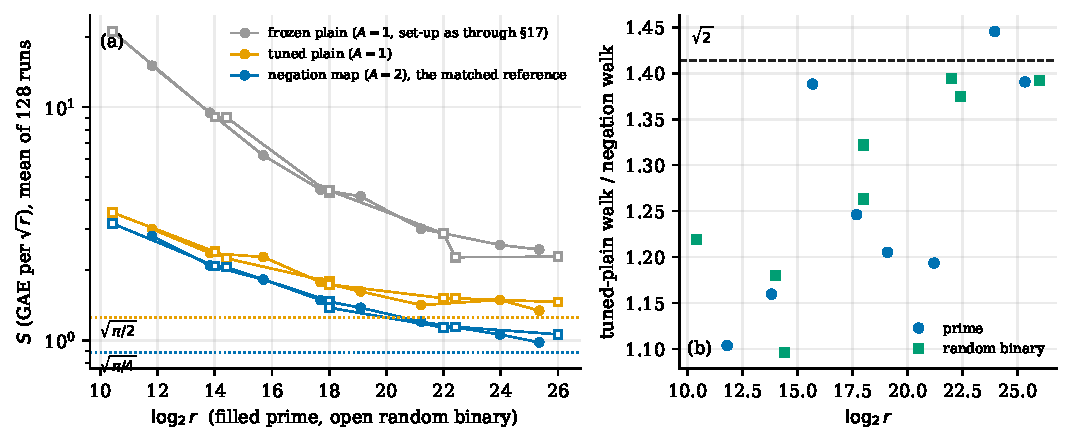
\includegraphics[width=\linewidth]{figures/fig-fr-rholadder.pdf}
\caption[]{The matched rho reference on its 16-curve evaluation ladder.
(a) Mean $S$ (GAE per $\sqrt r$, 128 runs) of the frozen plain walk, the
tuned plain walk and the negation-map walk; dotted lines: the plain and
negation floors $\sqrt{\pi/2}$ and $\sqrt{\pi/4}$. (b) Tuned-plain walk over
negation walk per curve, against $\sqrt2$ (dashed). Data:
\art{figures/data-fr-rholadder.json}, from
\art{research/ic_rho_reference_20260923/analysis.json}
(\texttt{tables.ladder}).}
\label{fig:fr-rholadder}
\end{figure}

\begin{table}[t]
\centering\scriptsize
\setlength{\tabcolsep}{3pt}
\begin{tabular}{@{}llrrrrrrrr@{}}
\toprule
regime & instance & $\log_2 r$ & $J$ & frozen & tuned plain & negation & neg.\ median & neg.\ walk/floor & plain/neg.\ walk \\
\midrule
prime & \texttt{generated-12bit-3529} & 11.81 & 4 & 15.05 & 3.000 & 2.801 & 2.573 & 1.727 & 1.104 \\
prime & \texttt{generated-14bit-14389} & 13.83 & 4 & 9.46 & 2.366 & 2.091 & 1.949 & 1.540 & 1.160 \\
prime & \texttt{generated-16bit-53411} & 15.70 & 8 & 6.21 & 2.275 & 1.821 & 1.753 & 1.235 & 1.388 \\
prime & \texttt{generated-18bit-212099} & 17.70 & 8 & 4.42 & 1.775 & 1.487 & 1.423 & 1.216 & 1.246 \\
prime & \texttt{generated-20bit-563153} & 19.10 & 8 & 4.14 & 1.619 & 1.378 & 1.289 & 1.272 & 1.205 \\
prime & \texttt{generated-22bit-2434423} & 21.22 & 8 & 3.01 & 1.415 & 1.201 & 1.189 & 1.197 & 1.193 \\
prime & \texttt{generated-24bit-16483309} & 23.97 & 16 & 2.56 & 1.490 & 1.058 & 1.039 & 1.075 & 1.445 \\
prime & \texttt{generated-26bit-42652151} & 25.35 & 16 & 2.45 & 1.339 & 0.979 & 0.909 & 1.024 & 1.391 \\
\addlinespace
char2 & \texttt{random-binary-n13-b168f} & 10.42 & 4 & 21.10 & 3.530 & 3.168 & 3.110 & 1.408 & 1.219 \\
char2 & \texttt{random-binary-n15-b157a} & 14.00 & 4 & 9.06 & 2.397 & 2.082 & 1.928 & 1.550 & 1.180 \\
char2 & \texttt{random-binary-n17-b10103} & 14.41 & 4 & 9.03 & 2.245 & 2.060 & 1.966 & 1.590 & 1.096 \\
char2 & \texttt{random-binary-n21-b968e} & 18.00 & 8 & 4.28 & 1.784 & 1.470 & 1.404 & 1.235 & 1.263 \\
char2 & \texttt{random-binary-n19-b770f7} & 18.00 & 8 & 4.39 & 1.735 & 1.380 & 1.316 & 1.141 & 1.322 \\
char2 & \texttt{random-binary-n23-b480f9a} & 22.00 & 16 & 2.87 & 1.514 & 1.134 & 1.111 & 1.047 & 1.395 \\
char2 & \texttt{random-binary-n25-b1a9b772} & 22.42 & 16 & 2.27 & 1.514 & 1.142 & 1.099 & 1.082 & 1.374 \\
char2 & \texttt{random-binary-n27-b227199e} & 26.00 & 16 & 2.28 & 1.459 & 1.060 & 1.061 & 1.127 & 1.392 \\
\bottomrule
\end{tabular}

\caption[]{The matched rho reference's evaluation ladder, every curve.
$J$: jumps in the tuned walks' table. Frozen, tuned plain, negation: mean
$S$ in GAE per $\sqrt r$ over 128 runs, whole solve; neg.\ median: median
$S$ of the negation walk. Neg.\ walk/floor: the negation walk's steps over
$\sqrt{\pi r/4}$. Plain/neg.\ walk: tuned plain walk over negation walk.
Source: \art{research/ic_rho_reference_20260923/analysis.json}. Data:
\art{figures/data-fr-rholadder.json}.}
\label{tab:fr-rholadder}
\end{table}

The toy excess therefore shrinks at medium size, as fixed set-up predicts,
but this is descriptive: no prime medium-tier rho bound exists in the plain
ECDLP domains of the frontier. Medium-tier \texttt{rho.negation} bounds
($1.114$ and $1.225\times$ the floor at 35.6--55.6 bits) exist only inside
the Cheon oracle domains, fitted on one tier of a mixed session and so
unranked (\S\ref{sec:gf-cheon}). The open step is to seal \texttt{rho.negation},
\texttt{rho.plain} and \texttt{bsgs.negation} at $\log_2r=32$--$48$ and fit
the toy-to-medium ratio
(\art{crypto-autoresearcher:knowledge/leads/ecdlp/generic/LEAD-RHO-matched-rho-calibration.yaml}).

\paragraph{Consequence.} Every prime-field distance in this treatise is
paired against rho on the same curve and in the same session, so the toy
excess sits in the denominator. Where both arms carry fixed set-up the
paired ratio is fair at that size; it does not transfer to another size,
and an exponent fitted over toy sizes inherits rho's sub-$\tfrac12$ slope.
This is why Chapter~\ref{ch:distance} quotes distances per size and fits
gap exponents only where the source does.

\section{The sealed frontier, version 1 and version 2}\label{sec:mr-frontier}

Bounds are sealed records of constant and exponent per method
(\S\ref{sec:ecbench}). The first frontier page named leaders that its data
did not support. The rebuild of 23 October under frontier procedure~2
(\art{research/ecbench_frontier_v2_20261023/}) is a \textbf{correction}:
no session ran; each of the 46 published v1 records stayed byte-identical
and gained a fit-version-2 twin; only v2 bounds fitted on four or more
curves of a whole session are ranked; and a leader is named only when its
interval separates from every other method's on shared curves.
Table~\ref{tab:mr-frontier} gives the change per domain.

\begin{table}[t]
\centering\small
\begin{tabularx}{\linewidth}{@{}l>{\raggedright}X>{\raggedright\arraybackslash}X@{}}
\toprule
Domain & v1 page & v2 page (current) \\
\midrule
prime toy & ops leader \texttt{bsgs.negation} ($1.100$ $[0.978,1.225]$) named on a point estimate & no ops leader: \texttt{bsgs.negation} and \texttt{rho.negation} ($1.453$ $[1.184,1.772]$) overlap, a tie set of six bounds; \texttt{rho.plain} ($1.920$) no longer dominated by \texttt{rho.negation} \\
Koblitz toy & leader a three-size tier-subset bound & no ops leader (tie set of three); both \texttt{rho.signed\_frobenius} bounds have a large tail (max/median $54.2$ and $11.7$) \\
Koblitz medium & ops leader strong rho & ops leader strong rho, $1.089$ $[0.927,1.261]$, $\alpha=0.451$ $[0.399,0.503]$, 144 runs, now separating on all six degrees; memory leader the pair claw \\
\bottomrule
\end{tabularx}
\caption[]{The bounds frontier before and after procedure~2. Source:
\art{research/ecbench_frontier_v2_20261023/README.md},
\art{docs/bounds/FRONTIER.md}.}
\label{tab:mr-frontier}
\end{table}

The v1 exponent intervals also carried degenerate ends from one-size
resamples; the kangaroo's $[0.179,2.500]$, on which ``$\alpha$ agrees with
declared'' rested, is $[0.401,0.724]$ in its v2 twin. Prime medium-tier
plain-ECDLP bounds are still absent (\S\ref{sec:mr-bias}).

\paragraph{The first challenge verdicts.} A bound moves the frontier only
through a verdict against a sealed challenge on frozen workloads. The first
two (\art{research/ecbench_bounds_challenges_20261006/}, epoch~1, 288 of
288 replays identical in each session, L0) were the reference challenges
themselves.
\begin{itemize}
\item \emph{Prime toy}: \texttt{bsgs.negation} against \texttt{rho.negation}
  reads \textbf{trade}, $0.8250$ $[0.725,0.945]$ of the operations at
  $15.79$ $[13.38,19.06]\times$ the table. No single curve's interval
  excludes 1; the pooled 96 pairs do.
\item \emph{Koblitz toy}: the lean \texttt{rho.signed\_frobenius} against the
  strong reference reads \textbf{advances} at the constant level, $0.2991$
  $[0.235,0.402]$ of the operations and $0.560$ of the table. It prices the
  strong walk's toy set-up and says nothing above $r=2^{24}$.
\end{itemize}
Neither moves an exponent. Both say which reference is ``strongest'' at
toy size depends on what is charged, which the band makes explicit.

\section{The band orders the references themselves}\label{sec:mr-band}

The pricing band of \S\ref{sec:band} was introduced to compare index
calculus with rho fairly. Applied to the rho references themselves, it
changes which of them is strongest.
\begin{itemize}
\item \emph{Negation against plain, prime toy.} \texttt{rho.negation} is
  better than \texttt{rho.plain} at the charged cost, but the order flips
  at $0.34$--$0.55$ GAE per unpriced canonicalisation, inside the band, so
  neither dominates (\art{docs/bounds/FRONTIER.md}). At 28--40 bits the
  negation audit finds the same: the order holds at $w=0$ and $0.1$; at
  $w=1$ the negation walk's $S$ is $1.89$--$2.03$, above plain, and the
  ranking is unresolved on all four curves
  (\art{research/rho_negation_audit_20261020/band.json}). A real
  canonicalisation is one $\FF_p$ negation and one comparison, far below
  1~GAE, but it was not priced.
\item \emph{Signed Frobenius against plain, Koblitz toy.} Dominance holds at
  the charged cost and flips at about $0.123$ GAE per uncharged operation;
  the kangaroo's dominance by signed-Frobenius and negation rho flips at
  $0.290$ and $0.417$.
\item \emph{Extension-field references.} Two references built for the
  extension-field programme use the full symmetry: \texttt{rho.gls}
  ($A=4$, GLS twists over $\FF_{p^2}$) and \texttt{rho.frobenius\_orbit}
  ($A=6$, $E/\FF_p$ on $E(\FF_{p^3})$), each on nine curves with 8 targets
  (\art{research/ext_endo_rho_20261023/analysis/}). At $w=0$ \texttt{rho.gls}
  costs $S=0.472$--$0.921$ against negation's $0.812$--$1.165$, and at $w=1$
  $2.316$--$4.197$ against $1.613$--$2.312$; every pair on every curve is
  unresolved inside the band. \texttt{rho.frobenius\_orbit} costs
  $0.482$--$0.692$ at $w=0$ against negation's $0.783$--$1.404$, and is below
  negation across the band on four of nine curves; on three curves
  \texttt{rho.plain} is below negation across the band.
\end{itemize}
The rule this implies is already in the gate's wording: a row's ``matched''
reference is the strongest available \emph{across the band}, and where the
references themselves are unresolved the row is ranked against each. A row
ranked against one weight's winner alone overstates index calculus at the
other weights.

\section{References that lacked the negation map}\label{sec:mr-negaudit}

The negation-map audit of 20 October
(\art{research/rho_negation_audit_20261020/}) inventoried every rho walk the
programme used as a reference. Two lacked the map: \texttt{volcano-rho}'s
native walk in this repository, and crypto-autoresearcher's
\texttt{index\_calculus/rho.py}. Both now walk on $\{R,-R\}$ by default.
This is a \textbf{correction of earlier references}: any index-calculus
ratio computed against either before 20 October was against a rho $\sqrt2$
weaker than the negation walk.
\begin{itemize}
\item \emph{The matched reference delivers the saving.} On four fresh
  prime-order curves of 28--40 bits (512 records, 16 exact replays),
  pooled plain over negation is $1.371$ $[1.257,1.491]$, with $\sqrt2$
  inside the interval.
\item \emph{Little of it reaches wall time} in ecbench's implementation:
  the median paired wall ratio is $1.140$ (L0, descriptive).
\item \emph{Per curve and per run} (Table~\ref{tab:fr-negaudit},
  Figure~\ref{fig:fr-collision}): the negation walk costs $0.953$--$1.016$
  and the plain walk $1.235$--$1.468$ at $w=0$; per-run cost follows the
  first-collision law of the Poisson model, shifted up by the walk's
  overhead (means $0.980$ and $1.343$ against $0.886$ and $1.253$). At
  $w=1$ the negation walk costs $1.892$--$2.029$, above plain on all four
  curves, so the band leaves the order unresolved on each.
\item \emph{\texttt{volcano-rho}.} On a 36-bit curve, 256 solves per arm,
  off over on is about $1.40$ pooled over five arms, at $9$--$16\%$ more
  nanoseconds per iteration (an extra branch, a field negation and a
  16-entry cycle-window scan), so wall time improves by about $1.2\times$.
\item \emph{crypto-autoresearcher.} 640 paired solves at 16--32 bits give
  plain over negation $1.353$ $[1.281,1.425]$; its adapter now labels the
  old walk \texttt{rho.plain} and refuses it as a matched reference.
\end{itemize}
An earlier fix in the collaborative walker
(\art{research/generic_dlp_correctness_20261017/}) found that its
negation-map 2-cycle test compared an unflipped sum with a normalised
point and never fired; dead trails fell from 353 to 16 across three
curves once it compared after the flip.

\begin{figure}[t]
\centering
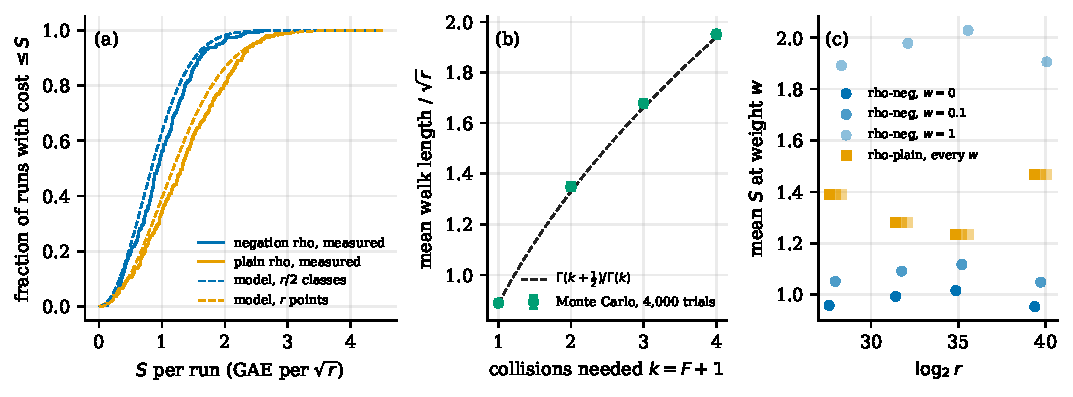
\includegraphics[width=\linewidth]{figures/fig-fr-collision.pdf}
\caption[]{Rho's collisions against the Gamma floor. (a) Per-run cost of
the negation-map and plain walks in the negation audit (256 runs each, four
prime-order curves of 28--40 bits, L0) against the first-collision law of
the Poisson model: $\Pr[S\le s]=1-e^{-s^2}$ on $r/2$ negation classes and
$1-e^{-s^2/2}$ on $r$ points (dashed; means $\sqrt{\pi/4}$ and
$\sqrt{\pi/2}$). (b) Monte Carlo mean of the $k$-th collision over $\sqrt r$
(4{,}000 trials, $r=131{,}203$) with $\pm1.96$ standard errors, against
$\Gamma(k+\tfrac12)/\Gamma(k)$ (Proposition~\ref{prop:collisionfloor}).
(c) Mean $S$ per curve at $w=0$, $0.1$ and~1 GAE per unpriced
canonicalisation; plain rho has none, so its three points coincide. Model
curves computed by \art{figures/make_fig_fr_collision.py}. Data:
\art{figures/data-fr-collision.json}, from
\art{research/rho_negation_audit_20261020/} (\texttt{comparisons},
\texttt{band.json}) and
\art{research/curve25519_rho_parity_bound_20261104/data/sim.json}.}
\label{fig:fr-collision}
\end{figure}

\begin{table}[t]
\centering\small
\setlength{\tabcolsep}{3.5pt}
\begin{tabular}{@{}lrlrrrrrl@{}}
\toprule
curve & $\log_2 r$ & arm & mean $S$ [95\%] & $S$/theory & wall ms & $w=0$ & $w=0.1$ & $w=1$ \\
\midrule
fp28 & 27.95 & rho-neg & 0.958 [0.846,1.076] & 1.081 & 7.6 & 0.958 & 1.051 & 1.892 \\
 &  & rho-plain & 1.391 [1.229,1.556] & 1.109 & 8.4 & 1.391 & 1.391 & 1.391 \\
 & & plain/neg. & 1.452 [1.223,1.717] & & & & & \\
\addlinespace
fp32 & 31.76 & rho-neg & 0.993 [0.884,1.108] & 1.120 & 17.8 & 0.993 & 1.091 & 1.979 \\
 &  & rho-plain & 1.280 [1.122,1.439] & 1.021 & 19.6 & 1.280 & 1.280 & 1.280 \\
 & & plain/neg. & 1.289 [1.113,1.496] & & & & & \\
\addlinespace
fp36 & 35.21 & rho-neg & 1.016 [0.895,1.140] & 1.146 & 55.2 & 1.016 & 1.117 & 2.029 \\
 &  & rho-plain & 1.235 [1.069,1.406] & 0.986 & 52.9 & 1.235 & 1.235 & 1.235 \\
 & & plain/neg. & 1.216 [1.013,1.450] & & & & & \\
\addlinespace
fp40 & 39.73 & rho-neg & 0.953 [0.821,1.096] & 1.075 & 223.1 & 0.953 & 1.048 & 1.906 \\
 &  & rho-plain & 1.468 [1.314,1.631] & 1.171 & 321.2 & 1.468 & 1.468 & 1.468 \\
 & & plain/neg. & 1.540 [1.289,1.851] & & & & & \\
\addlinespace
pooled & & plain/neg. & 1.371 [1.257,1.491] & & & & & \\
\bottomrule
\end{tabular}

\caption[]{The negation-map audit, per curve: 64 verified runs per arm and
curve, one session (\texttt{ECBS1h83b97eccdcda}, L0). Mean $S$ in GAE per
$\sqrt r$ with its 95\% interval; $S$/theory against $\sqrt{\pi/4}$ and
$\sqrt{\pi/2}$; wall: median ms per solve. $w$ columns: mean $S$ with each
unpriced canonicalisation charged $w$ GAE. Plain/neg.: paired ratio,
cluster 95\% interval. Sources:
\art{research/rho_negation_audit_20261020/table.md},
\art{research/rho_negation_audit_20261020/band.json},
\art{research/rho_negation_audit_20261020/sessions/negation_vs_plain/comparisons/rho-neg__rho-plain.json}.
Data: \art{figures/data-fr-collision.json}.}
\label{tab:fr-negaudit}
\end{table}

\paragraph{References that were not the strongest.} A register item of the
repair framework (\art{research/r12_rho_ns_per_step_20261026/}) listed every
committed ecbench spec that pairs an index-calculus arm with a rho arm:
745 specs in 68 directories, of which 37 directories pair index calculus
only with a rho other than the strong reference. On Koblitz curves, counted
ratios against \texttt{rho.negation}, \texttt{rho.plain} or the tuned
signed-Frobenius walk are therefore not matched to the strongest rho; on
prime curves \texttt{rho.negation} is the strongest reference. The same
note explains an audit's $599$ against $240$ ns per step: the unbatched
tuned rho is $5.48$, $9.34$ and $9.56\times$ slower per step than the strong
rho at $n=41,53,61$ (L0, Apple arm64, A/A within $\pm7\%$), and within the
strong algorithm the field backend matters by $1.07$--$1.76\times$ with the
hardware. The 599 ns figure being the tuned rho is a hypothesis supported
by the size match.

\section{Engineering the strong reference}\label{sec:mr-engineering}

Chapter~\ref{sec:frontier} records that the strong signed-Frobenius rho fell
from 1{,}196 to 718 instructions per step in three rounds, and that a fourth
round took \texttt{main} from 707.2 to 679.7 with no established native gain.
Table~\ref{tab:mr-rounds} gives the rounds; every round left walks, step
counts and recovered logarithms identical, so counted-unit records are
unchanged and only instruction or wall comparisons move.

\begin{table}[t]
\centering\small
\begin{tabularx}{\linewidth}{@{}l>{\raggedright}Xr>{\raggedright\arraybackslash}X@{}}
\toprule
Round & change & instr./step & native time \\
\midrule
canon (8 Oct) & longest-zero-run rotation search; scratch reuse & & $1.40\times$ per walk ($m=83$), $1.46$--$1.61\times$ ($n=41$--$61$) \\
Q4 (16 Oct) & changes declared in two addenda & $1{,}196\to938$ & $1.02\times$ ($n=53$), not established; $1.21\times$ ($n=61$) \\
canon2 (16 Oct) & six changes in the strong-rho source & $938\to781$ & \\
step3 (16 Oct) & target-feature walk; batched walk starts & $781\to718$ & \\
batchinv (22 Oct) & fixed-width batch inversion & $707.2\to679.7^{a}$ & not established \\
\bottomrule
\end{tabularx}
\caption[]{Engineering rounds on the strong Koblitz reference; instructions per walk step at $n=53$. Sources:
\art{research/strong_rho_canon_20261008/},
\art{research/rho_assurance_20261016/},
\art{research/rho_canon2_20261016/}, \art{research/rho_step3_20261016/},
\art{benchmarks/20261022-strong-rho-batchinv/} (carries a
\texttt{VALIDATION.json}; its validator passes the instruction reduction
and its findings contradict the native speed-up). $^{a}$From the \texttt{main} of 22 October, which already read $707.2$.}
\label{tab:mr-rounds}
\end{table}

The assurance round's Q3 profile motivated the rounds:
one step cost $1{,}196$ instructions, about 57 field multiplications,
against a floor near six or seven, and half of it was canonicalisation. A
separate optimisation of ecbench's standing method
(\art{research/ecbench_rho_optimized_20261014/}) cut complete-solve
Callgrind instructions to $0.802155$ of the trajectory-identical legacy
path, with charged GAE exactly $1.0000$ over 240 pairs and 720 of 720
replays identical; its native wall gate is unknown. The pattern is the
same in every round: counted GAE is the comparison unit and does not move;
wall-time comparisons against an older rho overstate index calculus by up
to the round's factor (Table~\ref{tab:audit-rho}).

\paragraph{Prime-field and GPU walks.} The batched affine step with
Montgomery's simultaneous inversion is the prime-field engineering baseline.
On P-256, a plain step costs 179~ns at 1{,}024 walks per inversion
(\art{research/rho_walk_leads_20261014/}). A branch-free $\FF_p$ 64-bit
kernel took \texttt{prime\_fast::rho\_parallel} from $98.9$ to $68.2$ ns per
step (\art{research/fp64_branchfree_20261016/}). An analytical model of
counted operations times measured cycles per operation predicted a batched
affine rho iteration to a median $1.8$--$5.5\%$ on five fields at
$B\ge4{,}096$ walks after one fitted residual per field
(\art{benchmarks/20261016-hwcost-rho-model/}). ECCp-131 throughput is in
Chapter~\ref{sec:prime}; GPU walks are in \S\ref{sec:rv-scale}.

\paragraph{Cheap jump tables.} Three ecbench variants build the
negation-map jump table more cheaply than \texttt{rho.negation}:
\texttt{rho.negation\_chained}, whose jumps satisfy
$M_j=M_{j-1}+M_{j-2}$, and the ladder tables \texttt{rho.negation\_v5} and
\texttt{\_v6}, which use $k\approx\sqrt F$ jumps and refuse every
three-term relation among them before spending an operation. One session
paired all four on six prime curves of $2^{17.7}$--$2^{28}$, 32 targets
$\times$ 6 rounds (1{,}152 pairs per comparison), with an A/A arm that read
$1.0000$ (\art{research/ecbench_rho_chained_vs_v5v6_20261111/}; L0, counted
GAE, 6{,}720 records verified, 5{,}760 replays reproduced; benchmark row with
a \texttt{VALIDATION.json} and an independent validator report, no
\texttt{pcc} claim). Table~\ref{tab:mr-jumps} gives the paired ratios. Both
cheap tables cut set-up to about $0.05\sqrt r$, but the chained table's
three-term relation becomes a short fruitless cycle under negation: cycle
escapes rise from $0.003\sqrt r$ to $0.045\sqrt r$ and the walk from
$1.009\sqrt r$ to $3.708\sqrt r$, while \texttt{v5} walks $0.884\sqrt r$
with rare escapes (270 of 1{,}152 runs, mean $0.0004\sqrt r$). Per curve,
chained over \texttt{rho.negation} rises from $1.75$ at $2^{17.7}$ to $7.62$
at $2^{28}$, in the direction of the chained method's own study, which had
rejected it. The validator found that chained and \texttt{rho.negation}
leave their distinguished-point probes undeclared while \texttt{v5} and
\texttt{v6} declare theirs; charging all at 1\,GAE gives \texttt{v5}/chained
$0.258$--$0.260$ and chained/\texttt{rho.negation} $3.38$--$3.40$, with no
ranking changed. The sealed bounds put \texttt{v5} at $1.103$ of the floor
($\alpha=0.461$) and \texttt{rho.negation} at $1.328$ ($\alpha=0.426$) over
these six sizes, below the calibrated range at four of them.

\begin{table}[t]
\centering\small
\begin{tabular}{@{}lll@{}}
\toprule
Comparison & paired ratio [95\%] & $w=0$ / $0.1$ / $1$ \\
\midrule
\texttt{v5} / chained & $0.256$ $[0.236,0.277]$ & $0.256$ / $0.257$ / $0.261$ \\
\texttt{v6} / chained & $0.261$ $[0.240,0.284]$ & $0.261$ / $0.263$ / $0.269$ \\
chained / \texttt{rho.negation} & $3.25$ $[2.98,3.54]$ & $3.25$ / $3.28$ / $3.42$ \\
\texttt{v5} / \texttt{rho.negation} & $0.831$ $[0.797,0.865]$ & $0.831$ / $0.841$ / $0.894$ \\
\texttt{v6} / \texttt{rho.negation} & $0.849$ $[0.814,0.885]$ & $0.849$ / $0.861$ / $0.919$ \\
\bottomrule
\end{tabular}
\caption[]{Negation-map rho with cheap jump tables, pooled over six prime
curves of $2^{17.7}$--$2^{28}$, counted GAE at L0. Every order holds across
the band. Measured on one local host; validated benchmark row
\art{benchmarks/20261111-rho-chained-vs-v5v6/}. Source:
\art{research/ecbench_rho_chained_vs_v5v6_20261111/reports/run-20261111T0324Z/REPORT.md}.}
\label{tab:mr-jumps}
\end{table}

A prime-field row matched to \texttt{rho.negation} at these sizes is
matched to a reference that \texttt{v5} undercuts by the factor in
Table~\ref{tab:mr-jumps}.

\paragraph{Harness overhead in small wall ratios.} Until 22 October ecbench
parsed its 4.7~MB curve registry on every lookup. Parsing it once cut the
timed solve window of every rho, BSGS and kangaroo arm to $0.03$--$0.07\times$
at 20 bits and $0.64$--$0.81\times$ at 32 bits, against $0.96\times$ for the
index-calculus pipeline (\art{benchmarks/20261022-ecbench-harness-overhead/},
which carries a \texttt{VALIDATION.json}; counted results unchanged). Any
small-size wall ratio recorded before then charged rho for about 4~ms of
harness work inside a 0.3~ms solve, which flattered index calculus.

\section{Formal assurance of the reference}\label{sec:mr-lean}

The strong reference is the denominator of every Koblitz row, so the
assurance round (\art{research/rho_assurance_20261016/}) checked its
correctness formally as well as empirically.
\begin{itemize}
\item \emph{Lean~4} (v4.34.1, no Mathlib): 34 theorems with no
  \texttt{sorry}, \texttt{admit} or \texttt{native\_decide}, using only
  \texttt{propext}, \texttt{Classical.choice} and \texttt{Quot.sound}. They
  cover the least-rotation canonicaliser (and its bridge to the Rust
  zero-run mask), Montgomery batch inversion in one- and four-accumulator
  forms over any field, and the walk algebra: starts, jumps,
  canonicalisation and escapes preserve $P=aG+bQ$, and the collision
  formula returns the logarithm whenever $b\ne b'$.
\item \emph{TLA+}: a model of the solve over $\ZZ_R$ meets all 41
  configurations' declared verdicts under TLC, including seven mutants that
  each fail the property meant to catch them.
\item \emph{Steps}: mean steps over $\sqrt{\pi r/(2A)}$ are $0.994$,
  $0.922$ and $0.943$ at $n=41,53,61$ on 400 fixtures each, with spread
  $0.50$--$0.51$ against an ideal random mapping's $0.52$.
\end{itemize}
The gaps are stated: the curve group is modelled as the scalar field, the
$\mathrm{GF}(2^m)$ arithmetic and basis maps are unverified, and word
overflow is argued, not proved. Four findings changed no answer; one (the
documented fruitless-cycle length) was a documentation fix.

Two further Lean files bear on rho's invariance
(\S\ref{sec:rv-isogeny}). \art{research/conductor_gap_rho_large_sample_20261018/lean/RepresentationHashInvariance.lean}
proves, in 11 theorems with no \texttt{sorry}, that transporting an
$r$-adding walk by a bijection compatible with the operation preserves its
trajectory and its cost at every budget, and that transport is a bijection
of walk spaces; so over a uniformly random partition rho's cost
distribution is the same on isomorphic groups, and a non-group invariant
can enter only through the one fixed hash an implementation uses.
\art{papers/isogeny-class-rho/lean/ScalarTransport.lean} proves (3
theorems) that a zero- and addition-preserving injective map transports
answers. Neither formalises curves or isogenies.

\section{Statistics version 2 and censored rho}\label{sec:mr-stats}

The statistics paragraph of \S\ref{sec:ecbench} describes the cluster
bootstrap of the original comparisons. PR~\#2442 replaced it with a
linearised $t(K-1)$ interval over $K$ workloads and, more consequentially,
kept timed-out and exhausted runs in the ratio as censored lower bounds
instead of dropping them (\art{research/ecbench_statistics_v2_20261105/};
no new runs).
\begin{itemize}
\item \emph{Width.} On uncensored rows the new interval is $13.1\times$
  wider at $K=2$, $1.23\times$ at $K=12$ and about $1.0$--$1.06\times$ at
  $K\ge16$. Its simulated coverage is $0.957$, $0.948$ and $0.947$ at
  $K=2,4,8$; the old percentile bootstrap covered $0.858$ at $K=2$ in the
  study's own simulation.
\item \emph{Censoring.} Dropping exhausted runs had understated
  \texttt{ic-sub6-mitm} over strong rho by $92.9\times$ ($6.981\to648.2$
  $[419.6,1001]$, a lower bound), and signed-Frobenius rho over
  \texttt{bsgs.negation} on a GHS panel by $60.4\times$ ($3.512\to212.0$),
  where 13 of the 40 workloads had exhausted rho runs.
\item \emph{The A/A gate.} Correcting a wall ratio by its A/A bias flipped
  one gating decision in the sample: \texttt{ic-sub6-mitm}'s ns per GAE
  ratio $1.248$ corrects to $1.147$ $[0.997,1.321]$, inside noise.
\end{itemize}
The rho-side lesson is the second item: an exhausted rho run is a failure
of the reference, and a comparison that drops it reads the reference as
cheaper than it was. Earlier ``$\times$ rho'' figures from sessions with
censored runs on either arm are lower or upper bounds accordingly.

\paragraph{Independence.} A same-machine replay under a different Rust
toolchain changed the environment class identifier and would have passed
the host-class part of an independent validation
(\art{research/ecbench_independence_20261009/}). A separate hardware class
that excludes toolchain, kernel and policy fields now rejects such a
receipt; the fingerprints remain self-reported, so an external runner's
custody record is still required.

\chapter{Walk design, memory and many targets}\label{ch:rhovariants}

The variations of rho the programme measured are: walks
on automorphism classes, the iteration function, rho across isogenous
curves and on Jacobians, the memory-heavy generic methods, many-target and
advice-table rho, and rho at deployed scale. Each moves the reference against which index calculus is ranked.

\section{Automorphism classes}\label{sec:rv-aut}

A walk on the classes of an efficiently computable automorphism group of
order $A$ saves $\sqrt A$ in steps, which is the ceiling for any
automorphism walk (\S\ref{sec:gf-shoup}); classes beyond $\mathrm{Aut}(E)$
are the open lead of \S\ref{sec:gf-advice}. The Koblitz signed-Frobenius
reference ($A=2n$) is the subject of Chapter~\ref{sec:koblitz}. On prime
curves the gains are smaller, and their measurement needed a correction.

\paragraph{$j=0$ and $j=1728$, with an erratum.} Round~2 of the conductor
gap had matched its crater rows against negation rho only. A follow-up ran
\texttt{rho.cubic} ($j=0$, $A=6$) and \texttt{rho.quartic} ($j=1728$, $A=4$)
on the same twelve crater curves
(\art{research/prime_rho_automorphism_20261015/}). Its \textbf{erratum of
24 October}: the binary left the class set-up (16--58 GAE per solve) out of
each record's total. Corrected,
\begin{itemize}
\item \texttt{rho.cubic}/\texttt{rho.negation} is $0.647$ $[0.543,0.770]$
  (was $0.611$), with the prediction $0.577$ inside;
\item \texttt{rho.quartic}/\texttt{rho.negation} is $0.819$ $[0.722,0.929]$
  (was $0.791$), whose interval no longer contains the prediction $0.707$.
\end{itemize}
Against the automorphism rho every crater IC/rho ratio of round~2 grows by
about $1.55\times$ ($j=0$) and $1.22\times$ ($j=1728$); that adjustment
applies pooled ratios and is not a joint re-run. The class-representative
map is unpriced, so the ratios do not bound full cost. The volcano-census
withdrawal of Chapter~\ref{ch:audit} is the same correction found from the
index-calculus side.

\paragraph{The crater is where the fold lives.} The volcano study
(\art{research/isogeny-volcano-rho/}) measured that the automorphism-folded
walk needs $1.89\pm0.09\times$ fewer operations on a $j=0$ crater ($\sqrt3$
predicted) and $1.32\pm0.06\times$ on a $j=1728$ crater ($\sqrt2$); in wall
time that is $1.33\times$ faster on $j=0$ and $2.3\times$ \emph{slower} on
$j=1728$, where the tool had no tuned walk. Across a whole $j=0$ class the
folded walk cost $0.439$ $[0.401,0.481]$ of the plain walk against
$1/\sqrt6=0.408$, and on the Koblitz crater the fold wins $1.7\times$ ($\tau$)
and $2.2\times$ ($\tau$ and negation) in wall time although each folded
step costs 41 squarings more (\art{research/isogeny-class-rho/REPORT.md}).
Every curve the isogenies lead to has lost the fold
(\S\ref{sec:rv-isogeny}).

\paragraph{GLS and $\FF_{p^3}$ references.} The extension-field references
and their band behaviour are in \S\ref{sec:mr-band}. On E25's ten GLS curves,
Karatsuba products with Montgomery-batched norm inversions cut the matched
$\langle\pm\psi\rangle$ walk's affine addition from 97 to $66.3$--$66.7$
$\FF_p$ multiplications, making it $1.453$--$1.463\times$ cheaper while the
index-calculus side moved only $1.0048$--$1.0057\times$; every row moved
further from rho, to $6.39\cdot10^3$--$4.06\cdot10^5\times$ at $w=0$
(\art{benchmarks/20261030-e27-walk-karatsuba/}, validated: independent
replay 11 of 11 runs, with errata in the validator report). It is a
correction to the reference, not an improvement.

\section{The negation map and fruitless cycles}\label{sec:rv-negation}

A negation walk creates fruitless 2-cycles $P\to P\pm R_i\to P$, and every
negation reference needs an escape. The walk-leads study
(\art{research/rho_walk_leads_20261014/}, Modal CPU, $N\approx2^{32}$--$2^{40}$)
measured the cycle rate and two representative rules.
\begin{itemize}
\item With a fixed or per-point rule the negation walk takes $1.37\times$
  $[1.31,1.43]$ and $1.33\times$ $[1.28,1.39]$ fewer steps than plain, with
  487 fruitless 2-cycles per $10^6$ steps against the predicted $1/(2r)=488$
  for $r=1{,}024$ jump points.
\item Changing the rule per epoch gives $0.83\times$ $[0.79,0.87]$: worse
  than no negation map.
\item Without an escape, every $\pm R$ arm repeats on a useless collision
  after $821$--$1{,}974$ steps against the plain walk's $69{,}210$ to a
  useful one at $N\approx2^{32}$: 0 or 1 of 200 solved.
\end{itemize}
The distributed pool of the sibling ecc-challenges repository walks plain
rho on all 23 non-ECC2K-130 campaigns. Its negation-class walk took $0.700$
$[0.673,0.728]$ of the old walk's steps with 0 of 1{,}800 trapped trails and
about $6\%$ per-step overhead, on toy curves of $2^{23}$--$2^{34.5}$; it is
in an open pull request as a post-hoc amendment, default off. These figures
are as the lead atlas reports them; that repository was not available to
this draft
(\art{crypto-autoresearcher:knowledge/leads/ecdlp/generic/LEAD-RHO-pool-class-quotient.yaml}).

\section{The iteration function}\label{sec:rv-mixing}

Chapter~\ref{sec:frontier} records the best-of-$P\pm R$ lead: $1.129\times$
fewer steps under distinguished points, offset by its cost per step. The
same study tested three more walk changes, and the in-degree argument
behind the first is the useful part.
\begin{itemize}
\item \emph{Best of $k$ candidates.} Choosing the best-scoring of $k$
  images gives a point of score rank $u$ the in-degree $ku^{k-1}$; since a
  random mapping's collision time scales as $1/\sqrt{\mathbb{E}[\lambda^2]}$,
  the predicted saving is $\sqrt{k^2/(2k-1)}$, $1.155$ for $k=2$ and $1.512$
  for $k=4$. A positive control hits it ($1.151$, $1.511$); under
  distinguished points best of four gives $1.463$ $[1.401,1.527]$ but costs
  $2.4$--$2.6\times$ a plain step, a net of about $0.6$.
\item \emph{Lazy reduction before the distinguished-point test}: no change
  ($0.998$ $[0.995,1.001]$); indexing the table on a lazy $x$ costs
  $0.733\times$, about the predicted $1/\sqrt2$.
\item \emph{Correlated walks.} A shared index sequence makes useful
  collisions impossible ($0.073\times$, with 176 of 1{,}000 trials
  censored); a precomputed pair table $R_i+R_j$ gives $1.027$
  $[0.982,1.073]$, since one addition still advances one step.
\end{itemize}

\paragraph{Mixing.} Teske's $r$-adding walks are near random for $r$ of 16
to 20. In the isogeny-class study the 32-adding walk ran at $1.0097$ of
$\sqrt{\pi n/2}$ on 4{,}400 solves against an expected $1.016$; a planted
4-adding walk read $1.291$ against Teske's $1.137$, and served as the
study's positive control (\art{research/isogeny-class-rho-n45/}). On
hyperelliptic Jacobians, mixing the divisor hash through a finaliser did
not reach its registered gains (\S\ref{sec:rv-jacobian}).

\paragraph{A compiled store-all schedule.} A theoretical current-plus-archive
walk $X_{t+1}=X_t+X_{t+1-d_t}$ with offsets compiled once per group order
(\art{research/tiered_rho_compiled_walk_20260921/}) has, exhaustively over
all 65{,}537 target logarithms at $2^{16}$, an exact capped mean of
$19{,}027{,}631/65{,}537$ additions against $19{,}114{,}086/65{,}537$ for the
matched unguided schedule: $0.4523\%$ fewer. It makes no wall-time claim.

\section{Rho across isogeny classes and volcano levels}\label{sec:rv-isogeny}

Chapter~\ref{ch:obstructions} proves that transport by an isogeny conserves
index-calculus cost, and Chapter~\ref{sec:transfer} records the volcano
census's level effects for index calculus. The generic twin is a measured
null: rho's cost does not depend on which isogenous curve, stratum or level
carries the instance.

\paragraph{One instance on every level.} \texttt{volcano-rho} carried one
instance ($p$ of 40 bits, $n=272{,}748{,}451{,}513$) by verified V\'elu
3-isogenies to all 80 curves of a depth-3 volcano and ran 100 paired-seed
solves on each of 29 curves and three isomorphic controls
(\art{research/isogeny-volcano-rho/}, benchmarks row
\texttt{20261016-isogeny-volcano-rho}; 32-adding walk, no negation).
Table~\ref{tab:rv-volcano} gives the levels.

\begin{table}[t]
\centering\small
\begin{tabular}{@{}lrrr@{}}
\toprule
Level & curves & solves & mean iterations $\pm$ 95\% \\
\midrule
0 (crater) & 2 & 200 & $700{,}483\pm47{,}849$ \\
1 & 6 & 600 & $681{,}766\pm26{,}525$ \\
2 & 10 & 1{,}000 & $637{,}158\pm20{,}410$ \\
3 (floor) & 11 & 1{,}100 & $659{,}589\pm20{,}993$ \\
all isogenous & 29 & 2{,}900 & $659{,}263\pm12{,}422$ \\
isomorphic control & 3 & 300 & $674{,}042\pm40{,}816$ \\
\bottomrule
\end{tabular}
\caption[]{Plain rho on one instance carried to every level of a 3-volcano
(curve~A, ramified crater), against $\sqrt{\pi n/2}=654{,}547$. Per-curve
means span $572{,}846$--$733{,}141$, the spread of 100-trial means of a
quantity with single-solve standard deviation about $341{,}000$; per-step
cost is $641$--$661$~ns on every curve. Source:
\art{research/isogeny-volcano-rho/README.md}.}
\label{tab:rv-volcano}
\end{table}

A control of 5{,}000 solves found that redrawing the secret, the generator
or both, or taking $k\le2^{16}$, matches the walk-seed spread (every
$\abs z<0.8$, Kolmogorov--Smirnov $p>0.6$).

\paragraph{Whole classes.} The isogeny-class study
(\art{research/isogeny-class-rho/}, protocol frozen before the run) ran
85{,}425 solves on 200 curves of four classes: 104 curves of a
347{,}004-curve prime-field class (12 endomorphism-ring strata, reached
through $\ell$-isogenies up to $\ell=61$), 45 curves of a $j=0$ class, 40
curves of a binary class and the Koblitz class over $\FF_{2^{41}}$. No
curve, stratum, level, isogeny degree or kernel-field degree left the
preregistered band, and the spread of means between curves is $1.1$--$1.2\times$
what the single-solve spread predicts. The 409- and 1{,}721-isogenies of
the Koblitz curve, whose division polynomials have degrees $83{,}640$ and
$1{,}480{,}920$, were found through torsion abscissae, and the curves they
reach cost $0.978$--$1.009$ of the reference by stratum. The detector works:
a planted negation fold read $0.63$--$0.77$ of the unfolded mean (expected
$0.71$). A 46-bit replica (4{,}400 solves on 38 curves) found pooled $1.0097$
against $1.016$ and Kruskal--Wallis $p=0.38$; one generator family flagged
there (KW $p=1.2\cdot10^{-4}$) \textbf{did not replicate} on a new draw (KW
$p=0.97$), and generator-level heterogeneity is recorded as unresolved
(\art{research/isogeny-class-rho-n45/README.md}; L0, no ecbench records, so
it supports no comparison claim).

\paragraph{A whole field.} The census of 11--12 November
(\art{research/fp31_whole_field_census_20261111/}; exact computations and
frozen-protocol runs, every result \texttt{[pcc:unverified]}, no
leaderboard row) took every isogeny class of $\FF_p$, $p=2^{31}-1$: one row
for each of the 185{,}363 traces, with $\sum_tH(4p-t^2)=2p$ curves exactly.
8{,}646 classes (4.66\%) have prime order and hold 2.64\% of the curves.
The only systematic cross-class effect is that larger classes have smoother
orders (Spearman $-0.141$ between $\log_2r$ and $\log_2H$), which is
Lenstra's divisibility bias, matched for every $\ell\le47$ to a relative
error of at most $1.3\cdot10^{-4}$. Weak classes are weak for textbook
reasons only, and no class with $r\ge2^{20}$ has embedding degree below 31.
Four measured phases followed (Table~\ref{tab:rv-fp31}). Counted rho cost
and IC relation yield do not depend on the class, its size, conductor,
number of endomorphism rings or $\abs{D_K}$, nor on the curve within a
class. In wall time per group operation a per-curve spread of about 1\% SD
remains after the curve order was randomised, but an isomorphic model of a
curve differs from it as much as an unrelated curve does, so the spread
belongs to the model and coordinates, not to the curve; the step formula
uses neither $a$ nor $b$, and the mechanism was not identified. The phase-5
rule requires a preregistered replication on fresh seeds before any model
is called cheaper.

\begin{table}[t]
\centering\footnotesize
\begin{tabularx}{\linewidth}{@{}>{\raggedright}p{1.9cm}>{\raggedright}p{2.3cm}>{\raggedright}X>{\raggedright\arraybackslash}p{2.1cm}@{}}
\toprule
Phase & population, scale & result & frozen verdict \\
\midrule
2: counted rho & 57 classes, 394 curves; 281{,}240 runs & normalised by $\sqrt{\pi r/2}$: Kruskal--Wallis $p=0.076$, Spearman $p\ge0.45$, per-class KS $p=0.20$; controls: planted fold $0.741$, A/A $1.003$, isomorphic $0.998$, $\sqrt r$ scaling $1.009$, $j=0$ fold $0.449$ (ideal $0.408$) & null supported \\
3: IC yield, $m=3$ and 2 & 48 classes, 332 curves; 526{,}111 relations & Kruskal--Wallis $p=0.58$, $0.64$; all 14 tests $p>0.05/14$; planted $+20\%$ reads $1.198$, $1.200$ & null supported \\
4: rho ns per GAE & 45 of 48 classes; 150{,}144 runs & within-class Friedman KS $p=3.5\cdot10^{-15}$; between-curve SD $0.95\%$; curve confounded with execution order & effect suspected; inconclusive \\
5: ns per GAE and per attempt, curve order randomised & 47--48 classes; 727 of 768 sessions & rho KS $p=7.7\cdot10^{-7}$, SD $0.91\%$, isomorphic-pair test $0.47$ (chance $0.5$, bar $0.75$); IC $p=0.48$, $0.62$ & rho: effect suspected, not intrinsic; IC: null \\
\bottomrule
\end{tabularx}
\caption[]{Rho and index calculus across the prime-order isogeny classes
of $\FF_{2^{31}-1}$. Phase 2 ran at L0; phases 4 and 5 graded most rows L2
on a local host. Sources:
\art{research/fp31_whole_field_census_20261111/README.md},
\art{research/fp31_whole_field_census_20261111/phase4/REPORT_PHASE4.typ},
\art{research/fp31_whole_field_census_20261111/phase5/REPORT_PHASE5.typ}.}
\label{tab:rv-fp31}
\end{table}

\paragraph{In ecbench.} A preregistered ecbench study on six 24-bit
volcanoes found rho's floor-over-crater ratio $1.022$ $[0.983,1.062]$ (90\%)
and BSGS identical on every curve and model; its v2 found rho $1.004$
(\art{benchmarks/20261017-isogeny-volcano-cost/},
\art{benchmarks/20261017-isogeny-volcano-cost-v2/}). The large-sample
floor/crater ratio of Chapter~\ref{sec:transfer} agrees. The Lean result of
\S\ref{sec:mr-lean} is the reason no effect was expected: over a random
partition, isomorphic groups give rho the same cost distribution.

\section{Rho on Jacobians}\label{sec:rv-jacobian}

Genus-2 and genus-3 transfer rows (Chapter~\ref{sec:transfer}) are ranked
against a distinguished-point rho on the same Jacobian, so that reference
needed its own calibration. Three rounds on 18 hyperelliptic instances
(genus 2--4, $N$ from 1{,}321 to $16{,}790{,}591$, 40 seeds each) tested it
in counted group operations.
\begin{itemize}
\item \emph{Negation fold.} Folded over plain is $0.67$--$0.89$ at
  $N\le6\cdot10^4$ but a median $0.968$ at $N\ge10^5$; the registered
  $\le0.80$ was falsified. Plain $S_{\text{walk}}$ was $1.82$ and $2.10$ at
  the two largest rows against an ideal $1.2533$
  (\art{benchmarks/20261018-hec-rho-negation/}).
\item \emph{Hash mixing.} Passing the divisor hash through a finaliser
  left the plain median at $1.406$ and fold over plain at $0.960$; both
  registered gains were falsified (\art{benchmarks/20261018-hec-rho-hash-mixing/}).
\item \emph{Branch width.} Full-width branch coefficients brought the
  median $S_{\text{walk}}$ at $N\ge10^5$ to $1.390$ and the largest row from
  $2.100$ to $1.481$ (\art{benchmarks/20261019-hec-rho-branch-width/}).
\end{itemize}
The third round is an accounting correction against index calculus: the
8-bit reference walk was slow at large $N$, so the early genus-2 to -4
ratios that read below rho are lower bounds (Chapter~\ref{sec:transfer}).

\section{Kangaroo, BSGS, the pair claw and store-all schedules}\label{sec:rv-memory}

\paragraph{Kangaroo.} \texttt{kangaroo.vow} is never an operations
leader: dominated on the prime toy tier, at $2.203$ $[1.803,2.527]\times$
its floor (\texttt{ECBND1h2e9e2024d8f3}) against negation rho's $1.453$;
unresolved inside the band on the Koblitz toy tier (the order against
signed-Frobenius and negation rho flips at about $0.290$ and $0.417$ GAE);
and unranked on the Koblitz medium tier, where $15.558$
$[13.742,17.597]\times$ its floor against signed-Frobenius rho's $1.188$ is
a three-size bound and a frontier entry needs four
(\art{docs/bounds/FRONTIER.md}). Its
calibration artefact of \S\ref{sec:mr-calibration} came from its
determinism per target. It is the right tool only for a known short
interval or a low-entropy secret
(\art{crypto-autoresearcher:knowledge/leads/ecdlp/generic/LEAD-RHO-kangaroo-interval.yaml}).

\paragraph{BSGS: fewer operations, more memory.} \texttt{bsgs.negation} is in
the prime toy tie set at $1.100$ $[0.978,1.225]\times$ the floor, the best
point estimate, but with $0.502\sqrt r$ table entries, which at 256 bits
is $2^{127}$. The challenge verdict of \S\ref{sec:mr-frontier} reads it as a
trade: $0.825$ of rho's operations at $15.8\times$ its table. The frontier names no
operations leader on the prime toy domain because the intervals overlap,
and the memory rules BSGS out at cryptographic size.

\paragraph{The pair claw is BSGS.} The four-point signed-Frobenius pair claw
of cryptanalysis~\#175 was ported into ecbench and run cold against the
strong rho on 48 one-target workloads over six Koblitz curves of
$2^{32.1}$--$2^{47.2}$ (\art{research/ecbench_pair_claw_20261003/}; 960 runs
verified, 12 of 12 replays identical, L0). Every factor-base logarithm is
known, so it is a randomised BSGS on signed-Frobenius classes, of cost
$(c+1/c)/\sqrt n$ against rho's $\sqrt{\pi/(4n)}$.
\begin{itemize}
\item At its cost-minimising shape ($c=1$) it costs $2.195$ $[1.897,2.546]$
  strong rho, and at the shape the pull request ran at $n=83$ it costs
  $32.65$ $[25.29,41.04]$. The ratio does not shrink with $r$.
\item Without the Frobenius fold, \texttt{bsgs.negation} costs $6.969$
  $[6.063,8.024]$ strong rho on the same workloads.
\end{itemize}
On the Koblitz medium frontier the claw at the pull request's shape is the
memory leader ($0.004\sqrt r$ entries, $35.6\times$ the floor), and the strong
rho the operations leader; the claw's other sealed shape ($2.390\times$ the
floor) is dominated by strong rho across the band. This is the $F=0$ exit of \S\ref{sec:gf-collision} in
practice.

\paragraph{Grumpy giants.} Bernstein and Lange's two grumpy giants and a baby
solve more targets per operation than BSGS or a random walk ($0.71875$
against $0.6753$ of targets at $1.5\sqrt\ell$). A certified exhaustive
ladder for its exact average-case constant ($\ZZ/\ell$, $2^{10}$--$2^{20}$)
has not run; its first stage met its support outcome at $\ell=101,257$
(\art{crypto-autoresearcher:knowledge/leads/ecdlp/generic/LEAD-RHO-grumpy-store-all-schedules.yaml}).
A certified constant below \texttt{bsgs.negation}'s would be a new toy
operations leader, and could not beat rho at cryptographic size, because
memory stays $\Theta(\sqrt\ell)$.

\section{Many targets: batch rho}\label{sec:rv-batch}

The one-target rule of \S\ref{sec:method} exists because many-target
figures were the easiest to misread. The Koblitz collection thread had
quoted every ``vs rho'' as the per-target cost of 32 targets solved
together, divided by rho solving one, and had counted each rho step and
each stored table pair as one addition. The repository's multi-target
margin rule makes batch rho at the same $k$ the reference for such a
figure, after Kuhn and Struik. A study frozen before it ran measured that
reference and priced both units (\art{research/ic_rho_koblitz_20260923/}).
\begin{itemize}
\item \emph{Batch rho.} $k$ targets solved in sequence by the tuned
  signed-Frobenius walk with one shared distinguished-point table. Per-target
  cost at $k=32$ over $k=1$ is $0.210$, $0.239$ and $0.190$ at $n=41,53,61$,
  each interval covering the Kuhn--Struik $0.199$; all $1{,}960$ targets
  were recovered and verified.
\item \emph{Prices in the thread's unit.} A canonical step costs
  $2.74$--$2.92$ units, Bailey et al.'s step $1.38$--$1.41$, and a stored pair
  $4.5$--$6.1$ ($6.14$ on the declared base).
\item \emph{The closest figure.} The thread's $1.17\times$ reads
  $6.51\times$ against batch rho as counted, $6.38\times$ with rho's step and
  the table build both priced, $12.6\times$ with Bailey's step on the
  canonical walk's count (a model), and $43.7\times$ for one target alone.
\end{itemize}
This is an \textbf{accounting correction}: no index-calculus count changed.
Its successor is Table~C of the Koblitz leaderboard, priced against batch
rho on the same 32 targets at $3.62$--$14.9\times$ and still pre-gate
(\S\ref{sec:tablea}).

\paragraph{Retention and distinguished points on prime curves.} The
multi-target index-calculus studies of \S\ref{sec:pg-multitarget} built the
two standard multi-target rhos in a counted field layer on prime-order
curves of $2^{22}$--$2^{32}$ and found that the reference itself needed
work. A rho that dropped the walk points of finished targets made a
multi-target IC look cheaper; Kuhn--Struik retention reversed that. The
first distinguished-point rho reused step values (about 39\% of its steps
duplicated another), so 1--34\% of its steps went to abandoned walks, and a
variant with distinct steps cost $0.81$--$0.99$ of it at $h=1$
(\art{research/mt_fieldops_v4_20261112/RESULTS.md}). Which multi-target rho
is cheapest depends on the price of a hash operation. In counted field
operations the retention rho wins at $h=0$ and $0.1$ in all 198 v5
configurations at $c_I=10$, often at the smallest database fraction of the
grid ($\kappa=0.05$); in wall time on one CPU the distinguished-point rho is
the fastest in 30 of 36 configurations. There a canonicalisation plus a
hash costs $0.005$--$0.009$\,GAE and a step index $0.002$--$0.006$\,GAE,
while a hash-table lookup costs up to $0.85$\,GAE at $2^{24}$ entries
(\art{research/mt_timed_20261112/RESULTS.md}).

\section{Advice tables}\label{sec:rv-advice}

Bernstein--Lange precomputation~\cite{bl2012} is the incumbent for every
online comparison; its use as the equal-advice control that retired the
online wins is in Chapter~\ref{ch:audit}, and the September decisions on
tables re-selected from the batch are in Chapter~\ref{ch:summer}. The
variants since then
(\art{crypto-autoresearcher:knowledge/leads/ecdlp/generic/LEAD-RHO-advice-table-variants.yaml})
add little.
\begin{itemize}
\item A table of $T/2$ entries re-selected from the batch's solved walks
  falls short of a static table of $T$ by $-0.064$ $[-0.080,-0.049]$ at
  $2^{24}$, contradicting its claim; a re-scoped selection at $0.65$--$0.75\,T$
  met its target in three of four toy cells (preliminary).
\item A basin-size instrument for table coverage failed its comparability
  gate.
\item Carrying a table across isogenous curves is exact and costs at most
  $1.3\%$ of a solve, but is never faster than solving at the source
  (\art{benchmarks/20261017-volcano-ecdlp-census/}).
\end{itemize}

\section{Rho at scale}\label{sec:rv-scale}

\paragraph{ECC2K-130.} The programme's GPU rho on ECC2K-130 is published
separately (\art{paper/ecc2k130/}); Chapter~\ref{sec:koblitz} prices the
index-calculus routes to it (\S\ref{sec:ecc2k130}). For the reference the
summary is this. The expected cost is $2^{60.9}$ iterations of a
Frobenius-class rho, and the walk constant was measured at
$2^{60.91}$--$2^{60.92}$. The $\sigma$-walk runs at $14.64$ billion
iterations per second on one RTX PRO~6000 in the audited campaign build
and $15.88$ in the best later build (a paired $1.0239\times$ over $15.51$,
A/A drift below $0.1\%$, 300 of 300 reports replayed;
\art{ecc2k130/SIGMA-TABLE.md}), about $230\times$ the 2010 GTX~295. A roofline
puts the ALU pipe at $91\%$ of its peak and the carry-less speed of light at
$27.4$ billion per second on that card (\art{ecc2k130/ROOFLINE.md}). The
paper separates the $\sigma$-walk from the table walk, whose $20.08$ was
measured under a cycle rule later found to leave cycles inconsistently;
the exact rule runs at $8.24$. A campaign stored 486 million distinguished
points and $2^{56.68}$ iterations ($5.4\%$ of the expected work) before its
fleet was reclaimed. Two iteration-function changes are derived and not
rolled out, because each starts a new distinguished-point corpus:
\begin{itemize}
\item signed $\sigma$ steps (\texttt{SIGMA\_SIGN=2}) need $0.958$--$0.967$ of
  the iterations at $n=41$ at a rate of $0.9965$, for $0.961$--$0.970$ of the
  time per solve (\art{benchmarks/20261014-ecc2k130-signed-sigma/});
\item a table walk with every fruitless cycle caught is projected at
  $0.81$--$0.86\times$ the $\sigma$-walk's cost per solve, unmeasured on the
  current kernel (\art{ecc2k130/WALK-CONSTANT.md}).
\end{itemize}
An audit of the live walk measured $2^{28.41}$ steps per completed walk at
the $\mathrm{HW}(x)\le32$ cutoff and added duplicate-point, seed-reset and
fruitless-cycle guards (\art{research/ecc2k130_rho_audit_20260925/}).
None of this improves on the generic bound, and the paper says so.

\paragraph{NIST P-256 and P-384 on a GPU.} The same levers applied to the
\texttt{gpu/nist} engine took P-256 from $1.075$ to $1.632$ and P-384 from
$0.210$ to $0.548$ billion iterations per second on one RTX PRO~6000
($1.52\times$ and $2.61\times$), through PTX carry chains and a batch width
$W=32$ with by-reference inversion (\art{benchmarks/20261013-nist-gpu-rho-ladder/};
single-run sweep cells, no isolation receipt). An inversion-free Jacobian
seeding ladder cut P-256 walk seeding from $11.53$ to $0.66$~ms per seed
($17.4\times$), a set-up change with the step unchanged
(\art{benchmarks/20261017-gpu-nist-jac-seed/}). At these rates P-256 remains
about $6\cdot10^{21}$ card-years away (\art{paper/ecc2k130/}). No GPU arm is
admitted to ecbench, because the matched-workload contract lacks PCIe
telemetry and an admission rule
(\art{problems/ecbench-gpu-matched-workload-contract.md}), and a P-256
best-of-two distinguished-point deficit remains unattributed, with its
$0.947$ cost estimate derived, not measured
(\art{problems/nist-best2-dp-bias-and-gpu-validation.md}).

\paragraph{Reading.} At scale the reference is an engineering artefact as
much as an algorithm: its constant is measured, its throughput is set by a
pipe, and each walk change has a corpus cost. None of it moves the generic
exponent. All of it moves the denominator of every index-calculus row,
which is why the gate of \S\ref{sec:gate} names the reference per row and
why a row ranked against a reference that has not adopted a change
overstates index calculus by that change's factor.
